\documentclass[
  shortnames]{jss}

%% recommended packages
\usepackage{orcidlink,thumbpdf,lmodern}

\usepackage[utf8]{inputenc}

\author{
H. Sherry Zhang\\Monash University \And Dianne Cook\\Monash University \And Ursula Laa\\University of Natural \\ Resources and Life Sciences \AND Nicolas Langrené\\BNU-HKBU \\ United International College \And Patricia Menéndez\\Monash University
}
\title{\pkg{cubble}: An \proglang{R} Package for Organizing and Wrangling Multivariate Spatio-temporal Data}

\Plainauthor{H. Sherry Zhang, Dianne Cook, Ursula Laa, Nicolas Langrené, Patricia Menéndez}
\Plaintitle{cubble: An R Package for Organizing and Wrangling Multivariate Spatio-temporal Data}


\Abstract{
Multivariate spatio-temporal data refers to multiple measurements taken across space and time. For many analyses, spatial and time components can be separately studied: for example, to explore the temporal trend of one variable for a single spatial location, or to model the spatial distribution of one variable at a given time. However for some studies, it is important to analyze different aspects of the spatio-temporal data simultaneously, like for instance, temporal trends of multiple variables across locations. In order to facilitate the study of different portions or combinations of spatio-temporal data, we introduce a new class, \code{cubble}, with a suite of functions enabling easy slicing and dicing on different spatio-temporal components. The proposed \code{cubble} class ensures that all the components of the data are easy to access and manipulate while providing flexibility for data analysis. In addition, the \pkg{cubble} package facilitates visual and numerical explorations of the data while easing data wrangling and modelling. The \code{cubble} class and the tools implemented in the package are illustrated with different examples of Australian climate data.
}

\Keywords{spatial, temporal, spatio temporal, \proglang{R}, environmental data, exploratory data analysis}
\Plainkeywords{spatial, temporal, spatio temporal, R, environmental data, exploratory data analysis}

%% publication information
%% \Volume{50}
%% \Issue{9}
%% \Month{June}
%% \Year{2012}
%% \Submitdate{}
%% \Acceptdate{2012-06-04}

\Address{
    H. Sherry Zhang\\
    Monash University\\
    21 Chancellors Walk, Clayton VIC 3800 Australia\\
  E-mail: \email{huize.zhang@monash.edu}\\
  
      Dianne Cook\\
    Monash University\\
    21 Chancellors Walk, Clayton VIC 3800 Australia\\
  E-mail: \href{mailto:dicook@monash.edu}{\nolinkurl{dicook@monash.edu}}\\
  
      Ursula Laa\\
    University of Natural \\ Resources and Life Sciences\\
    Gregor-Mendel-Straße 33, 1180 Wien, Austria\\
  E-mail: \href{mailto:ursula.laa@boku.ac.at}{\nolinkurl{ursula.laa@boku.ac.at}}\\
  
      Nicolas Langrené\\
    BNU-HKBU \\ United International College\\
    2000 Jintong Road, Tangjiawan, Zhuhai, Guangdong Province, China\\
  E-mail: \href{mailto:nicolaslangrene@uic.edu.cn}{\nolinkurl{nicolaslangrene@uic.edu.cn}}\\
  
      Patricia Menéndez\\
    Monash University\\
    21 Chancellors Walk, Clayton VIC 3800 Australia\\
  E-mail: \href{mailto:patricia.menendez@monash.edu}{\nolinkurl{patricia.menendez@monash.edu}}\\
  
  }

% Pandoc syntax highlighting
\usepackage{color}
\usepackage{fancyvrb}
\newcommand{\VerbBar}{|}
\newcommand{\VERB}{\Verb[commandchars=\\\{\}]}
\DefineVerbatimEnvironment{Highlighting}{Verbatim}{commandchars=\\\{\}}
% Add ',fontsize=\small' for more characters per line
\usepackage{framed}
\definecolor{shadecolor}{RGB}{248,248,248}
\newenvironment{Shaded}{\begin{snugshade}}{\end{snugshade}}
\newcommand{\AlertTok}[1]{\textcolor[rgb]{0.94,0.16,0.16}{#1}}
\newcommand{\AnnotationTok}[1]{\textcolor[rgb]{0.56,0.35,0.01}{\textbf{\textit{#1}}}}
\newcommand{\AttributeTok}[1]{\textcolor[rgb]{0.77,0.63,0.00}{#1}}
\newcommand{\BaseNTok}[1]{\textcolor[rgb]{0.00,0.00,0.81}{#1}}
\newcommand{\BuiltInTok}[1]{#1}
\newcommand{\CharTok}[1]{\textcolor[rgb]{0.31,0.60,0.02}{#1}}
\newcommand{\CommentTok}[1]{\textcolor[rgb]{0.56,0.35,0.01}{\textit{#1}}}
\newcommand{\CommentVarTok}[1]{\textcolor[rgb]{0.56,0.35,0.01}{\textbf{\textit{#1}}}}
\newcommand{\ConstantTok}[1]{\textcolor[rgb]{0.00,0.00,0.00}{#1}}
\newcommand{\ControlFlowTok}[1]{\textcolor[rgb]{0.13,0.29,0.53}{\textbf{#1}}}
\newcommand{\DataTypeTok}[1]{\textcolor[rgb]{0.13,0.29,0.53}{#1}}
\newcommand{\DecValTok}[1]{\textcolor[rgb]{0.00,0.00,0.81}{#1}}
\newcommand{\DocumentationTok}[1]{\textcolor[rgb]{0.56,0.35,0.01}{\textbf{\textit{#1}}}}
\newcommand{\ErrorTok}[1]{\textcolor[rgb]{0.64,0.00,0.00}{\textbf{#1}}}
\newcommand{\ExtensionTok}[1]{#1}
\newcommand{\FloatTok}[1]{\textcolor[rgb]{0.00,0.00,0.81}{#1}}
\newcommand{\FunctionTok}[1]{\textcolor[rgb]{0.00,0.00,0.00}{#1}}
\newcommand{\ImportTok}[1]{#1}
\newcommand{\InformationTok}[1]{\textcolor[rgb]{0.56,0.35,0.01}{\textbf{\textit{#1}}}}
\newcommand{\KeywordTok}[1]{\textcolor[rgb]{0.13,0.29,0.53}{\textbf{#1}}}
\newcommand{\NormalTok}[1]{#1}
\newcommand{\OperatorTok}[1]{\textcolor[rgb]{0.81,0.36,0.00}{\textbf{#1}}}
\newcommand{\OtherTok}[1]{\textcolor[rgb]{0.56,0.35,0.01}{#1}}
\newcommand{\PreprocessorTok}[1]{\textcolor[rgb]{0.56,0.35,0.01}{\textit{#1}}}
\newcommand{\RegionMarkerTok}[1]{#1}
\newcommand{\SpecialCharTok}[1]{\textcolor[rgb]{0.00,0.00,0.00}{#1}}
\newcommand{\SpecialStringTok}[1]{\textcolor[rgb]{0.31,0.60,0.02}{#1}}
\newcommand{\StringTok}[1]{\textcolor[rgb]{0.31,0.60,0.02}{#1}}
\newcommand{\VariableTok}[1]{\textcolor[rgb]{0.00,0.00,0.00}{#1}}
\newcommand{\VerbatimStringTok}[1]{\textcolor[rgb]{0.31,0.60,0.02}{#1}}
\newcommand{\WarningTok}[1]{\textcolor[rgb]{0.56,0.35,0.01}{\textbf{\textit{#1}}}}

% tightlist command for lists without linebreak
\providecommand{\tightlist}{%
  \setlength{\itemsep}{0pt}\setlength{\parskip}{0pt}}

% From pandoc table feature
\usepackage{longtable,booktabs,array}
\usepackage{calc} % for calculating minipage widths
% Correct order of tables after \paragraph or \subparagraph
\usepackage{etoolbox}
\makeatletter
\patchcmd\longtable{\par}{\if@noskipsec\mbox{}\fi\par}{}{}
\makeatother
% Allow footnotes in longtable head/foot
\IfFileExists{footnotehyper.sty}{\usepackage{footnotehyper}}{\usepackage{footnote}}
\makesavenoteenv{longtable}



\usepackage{amsmath} \usepackage{array}

\begin{document}



\hypertarget{introduction}{%
\section{Introduction}\label{introduction}}

Spatio-temporal data has a spatial component referring to the location of each observation and a temporal component that is recorded at regular or irregular time intervals. It may also include multiple variables measured at each spatial and temporal values. With spatio-temporal data, one can fix the time to explore the spatial features of the data, fix the spatial location/s to explore temporal aspects, or dynamically explore the space and time simultaneously.

In order to computationally explore the spatial, temporal and spatio-temporal faces of such data, the data needs to be stored and represented under a specific data object that allows the user to query, group and dissect all the data faces.

The Comprehensive \proglang{R} Archive Network (CRAN) task view SpatioTemporal \citep{ctvspatiotemporal} gathers information about \proglang{R} packages designed for spatio-temporal data and it has a section on \emph{Representing data} that lists existing spatio-temporal data representations used in \proglang{R}. Among them, the \pkg{spacetime} package \citep{spacetime} implements four S4 classes to handle spatio-temporal data with different spatio-temporal layouts (full grid, sparse grid, irregular, and trajectory). The \pkg{stars} package \citep{stars} implements an S3 class built from dense arrays.

Still, these two implementations are not necessarily easy to work in analysis for analysts with a tidyverse mindset. In tidyverse, data are in tables and the tidy data concept \citep{tidydata} prescribes three principles on how data should be organised for easier analysis as 1) one observation a row, 2) one variable a column, and 3) one type of observation a table. The third principle of tidy data is particularly relevant for spatio-temporal data since spatial and temporal data are naturally observed at different units: the location and location at different times. While the tidyverse suite implements data wrangling and visualisation tools operated on a single table, there has not been many tools for handling relational data for spatio-temporal analysis. This motivates a new design to organise spatio-temporal data in a way that would make data wrangling, visualizing and analyzing easier.

This paper presents a new \proglang{R} package, \pkg{cubble}, which implements a new cubble class to organize spatial and temporal variables as two forms of a single data object so that they can be wrangled separately or combined, while being kept synchronized. Among the four spacetime layouts in \citet{spacetime}, the \code{cubble} class can handle the full grid layout and the sparse grid layout. The software is available from the Comprehensive \proglang{R} Archive Network (CRAN) at \url{https://CRAN.R-project.org/package=cubble}.

The rest of the paper is organized as follows: Section \ref{cubble} presents the main design and functionality of the \pkg{cubble} package. Section \ref{others} explains how the \pkg{cubble} package deals with more advanced considerations, including data matching and how the package fits with existing static and interactive visualization tools. Moreover we also illustrate how the \pkg{cubble} package deals with spatio-temporal data transformations. Section \ref{examples} uses primarily Australian weather station data as examples to demonstrate the use of the package. An example of how the \pkg{cubble} package handles Network Common Data Form (NetCDF) data is also provided. Section \ref{conclude} discuss the paper contributions and future directions.

\hypertarget{cubble}{%
\section{The cubble package}\label{cubble}}

\hypertarget{object}{%
\subsection{The cubble object}\label{object}}

Spatio-temporal data can encompass data with various spatial and temporal characteristics and different data require different structures for wrangling and analysis: climate weather stations record data at fixed point location but may suffer from potential temporal data quality issue such as missing data for certain days. GPS data tracks unique point locations at different timestamps and is represented as trajectories. Satellite imageries capture snapshots of landscapes at selected time and is commonly structured as raster data. The spatio-temporal data cubble address are those collected at unique fixed locations while allowing for irregularity in the temporal dimension, such as the weather station data.

The cubble class is an S3 class built on tibble that allows the spatio-temporal data to be wrangled in two forms: a nested form (spatial cubble) and a long form (temporal cubble). It consists of two subclasses:

\begin{itemize}
\tightlist
\item
  a spatial cubble with class \texttt{c("spatial\_cubble\_df",\ "cubble\_df")}
\item
  a temporal cubble with class \texttt{c("temporal\_cubble\_df",\ "cubble\_df")}
\end{itemize}

In a spatial cubble, spatial variables are organised as columns and temporal variables are nested within a specialised \texttt{ts} column. The cubble object printed below contains weather records in three airport stations (the creation of a cubble object will be explained in Section \ref{create}). This toy data is a subset of a larger data \code{climate_aus} collected from Global Historical Climatology Network Daily (GHCND). It records three airport stations located in Melbourne, Australia and includes spatial variables such as station ID, longitude, latitude, elevation, station name, World Meteorology Organisation ID. The dataset contains temporal variables including precipitation, maximum and minimum temperature, which can be read from the cubble header:

\begin{CodeChunk}
\begin{CodeInput}
R> cb_nested
\end{CodeInput}
\begin{CodeOutput}
# cubble:   key: id [3], index: date, nested form
# spatial:  [144.8321, -37.98, 145.0964, -37.6655], Missing CRS!
# temporal: date [date], prcp [dbl], tmax [dbl], tmin [dbl]
  id           long   lat  elev name              wmo_id ts               
  <chr>       <dbl> <dbl> <dbl> <chr>              <dbl> <list>           
1 ASN00086038  145. -37.7  78.4 essendon airport   95866 <tibble [10 x 4]>
2 ASN00086077  145. -38.0  12.1 moorabbin airport  94870 <tibble [10 x 4]>
3 ASN00086282  145. -37.7 113.  melbourne airport  94866 <tibble [10 x 4]>
\end{CodeOutput}
\end{CodeChunk}

In a temporal cubble, temporal variables are expanded in the long form and spatial variables are stored as a data attribute:

\begin{CodeChunk}
\begin{CodeInput}
R> cb_long
\end{CodeInput}
\begin{CodeOutput}
# cubble:   key: id [3], index: date, long form
# temporal: 2020-01-01 -- 2020-01-10 [1D], no gaps
# spatial:  long [dbl], lat [dbl], elev [dbl], name [chr], wmo_id [dbl]
  id          date        prcp  tmax  tmin
  <chr>       <date>     <dbl> <dbl> <dbl>
1 ASN00086038 2020-01-01     0  26.8  11  
2 ASN00086038 2020-01-02     0  26.3  12.2
3 ASN00086038 2020-01-03     0  34.5  12.7
4 ASN00086038 2020-01-04     0  29.3  18.8
5 ASN00086038 2020-01-05    18  16.1  12.5
# i 25 more rows
\end{CodeOutput}
\end{CodeChunk}

\hypertarget{the-cubble-attributes}{%
\subsubsection{The cubble attributes}\label{the-cubble-attributes}}

A cubble object inherits the attributes from tibble (and its subclasses): \texttt{class}, \texttt{row.names}, and \texttt{names}. Additionally, it has three specialised attributes: \texttt{key}, \texttt{index}, and \texttt{coords}. Readers who are familiar with the \texttt{key} and \texttt{index} attributes from the \texttt{tsibble} package would already understand the two arguments. In cubble, the \texttt{key} attribute identifies the row in the spatial cubble (given the use of \texttt{tidyr::nest()} for nesting), and when combined with the \texttt{index} argument, it identifies the row in the temporal cubble. Currently, cubble only supports one variable as the key, and the accepted temporal classes for index includes the base R classes \texttt{Date}, \texttt{POSIXlt}, \texttt{POSIXct}, as well as tsibble's \texttt{yearmonth}, \texttt{yearweek}, and \texttt{yearquarter} classes.

The \texttt{coords} attribute represents an ordered pair of coordinates. It can be either an unprojected pair of longitude and latitude, or a projected easting and northing value. The \texttt{sf} package is used under the hood to calculate the bounding box, displayed in the header of a spatial cubble.

The temporal cubble has a special attribute called \texttt{spatial} to store the spatial variables. Shortcut functions are available to extract attributes, for example, \code{spatial()} for extracting spatial variables from the temporal cubble:

\begin{CodeChunk}
\begin{CodeInput}
R> spatial(cb_long)
\end{CodeInput}
\begin{CodeOutput}
# A tibble: 3 x 6
  id           long   lat  elev name              wmo_id
  <chr>       <dbl> <dbl> <dbl> <chr>              <dbl>
1 ASN00086038  145. -37.7  78.4 essendon airport   95866
2 ASN00086077  145. -38.0  12.1 moorabbin airport  94870
3 ASN00086282  145. -37.7 113.  melbourne airport  94866
\end{CodeOutput}
\end{CodeChunk}

\hypertarget{create}{%
\subsection{Creation and coercion}\label{create}}

In many cases, spatio-temporal data arrive in separate tables for analysis. For example, in climate data, analysts may initially receive station data containing geographic location information, recorded variables and their recording periods. They can then query the temporal variables using the stations of interest to obtain the relevant temporal data. Alternatively, analyses may begin as purely spatial or temporal, and analysts may obtain additional temporal or spatial data to expand the result to spatio-temporal.

The function \code{make_cubble()} composes a \code{cubble} object from a spatial table (\code{spatial}) and a temporal table (\code{temporal}), along with three attributes introduced in the subsection \ref{object}: \code{key}, \code{index}, and \code{coords}. The following code creates the spatial \code{cubble} object shown previously:

\begin{CodeChunk}
\begin{CodeInput}
R> make_cubble(spatial = stations, temporal = meteo,
+             key = id, index = date, coords = c(long, lat))
\end{CodeInput}
\end{CodeChunk}

Spatio-temporal data in other foreign objects can be coerced into a \code{cubble} object with the function \code{as_cubble()}. This includes casting from a \code{tibble} or \code{data.frame} with both spatial and temporal information, a NetCDF object, a \code{stars} object \citep{stars}, and a \code{sftime} object \citep{sftime}. The two examples below show the casting from a tibble and a NetCDF object. The dataset \code{climate_flat} combines the spatial data, \code{stations}, with the temporal data, \code{meteo}, into a single tibble object. It can be coerced into a cubble using:

\begin{CodeChunk}
\begin{CodeInput}
R> climate_flat |> as_cubble(key = id, index = date, coords = c(long, lat))
\end{CodeInput}
\begin{CodeOutput}
# cubble:   key: id [3], index: date, nested form
# spatial:  [144.8321, -37.98, 145.0964, -37.6655], Missing CRS!
# temporal: date [date], prcp [dbl], tmax [dbl], tmin [dbl]
  id           long   lat  elev name              wmo_id ts               
  <chr>       <dbl> <dbl> <dbl> <chr>              <dbl> <list>           
1 ASN00086038  145. -37.7  78.4 essendon airport   95866 <tibble [10 x 4]>
2 ASN00086077  145. -38.0  12.1 moorabbin airport  94870 <tibble [10 x 4]>
3 ASN00086282  145. -37.7 113.  melbourne airport  94866 <tibble [10 x 4]>
\end{CodeOutput}
\end{CodeChunk}

\hypertarget{functions-and-methods}{%
\subsection{Functions and methods}\label{functions-and-methods}}

Table \ref{tab:funs} summarises the functions implemented in the \pkg{cubble} package and Table \ref{tab:methods} details the methods implemented for each of the three cubble classes. The \code{cubble_df} class handles methods that behave consistently in both spatial (\code{spatial_cubble_df}) and temporal cubble (\code{temporal_cubble_df}). When the method has distinct behavior for the spatial cubble and temporal cubble, it is implemented separately for each subclass.

\begin{longtable}[]{@{}
  >{\raggedright\arraybackslash}p{(\columnwidth - 2\tabcolsep) * \real{0.1250}}
  >{\raggedright\arraybackslash}p{(\columnwidth - 2\tabcolsep) * \real{0.8750}}@{}}
\caption{\label{tab:funs} An overview of functions implemented in the \pkg{cubble} package, categorised into base R, tidyverse, and cubble functions.}\tabularnewline
\toprule()
\begin{minipage}[b]{\linewidth}\raggedright
Category
\end{minipage} & \begin{minipage}[b]{\linewidth}\raggedright
Functions
\end{minipage} \\
\midrule()
\endfirsthead
\toprule()
\begin{minipage}[b]{\linewidth}\raggedright
Category
\end{minipage} & \begin{minipage}[b]{\linewidth}\raggedright
Functions
\end{minipage} \\
\midrule()
\endhead
base R & \texttt{{[}}, \texttt{{[}{[}\textless{}-}, \texttt{names\textless{}-} \\
tidyverse & \texttt{dplyr\_row\_slice}, \texttt{dplyr\_col\_modify}, \texttt{dplyr\_reconstruct}, \texttt{select}, \texttt{mutate}, \texttt{arrange}, \texttt{filter}, \texttt{group\_by}, \texttt{ungroup}, \texttt{summarise}, \texttt{select}, \texttt{slice}, \texttt{rowwise}, \texttt{rename}, \texttt{bind\_rows}, \texttt{bind\_cols}, \texttt{relocate}, \texttt{type\_sum}, the slice family (\texttt{slice\_head}, \texttt{slice\_tail}, \texttt{slice\_max}, \texttt{slice\_min}, \texttt{slice\_sample}) and the join family (\texttt{left\_join}, \texttt{right\_join}, \texttt{inner\_join}, \texttt{full\_join}, \texttt{anti\_join}, \texttt{semi\_join}) \\
cubble & \texttt{as\_cubble}, \texttt{cubble}, \texttt{make\_cubble}, \texttt{check\_key} \texttt{face\_temporal}, \texttt{face\_spatial}, \texttt{unfold}, \texttt{key}, \texttt{key\_vars}, \texttt{key\_data}, \texttt{index}, \texttt{index\_var}, \texttt{coords}, \texttt{spatial}, \texttt{match\_sites}, \texttt{match\_spatial}, \texttt{match\_temporal}, \texttt{geom\_glyph}, \texttt{geom\_glyph\_box}, \texttt{geom\_glyph\_line}, \texttt{make\_spatial\_sf}, \texttt{make\_temporal\_tsibble}, \texttt{fill\_gaps}, and \texttt{scan\_gaps} \\
\bottomrule()
\end{longtable}

\begin{longtable}[]{@{}
  >{\raggedright\arraybackslash}p{(\columnwidth - 2\tabcolsep) * \real{0.2500}}
  >{\raggedright\arraybackslash}p{(\columnwidth - 2\tabcolsep) * \real{0.7500}}@{}}
\caption{\label{tab:methods} An overview of the methods implemented in the three \code{cubble} classes. Methods are implemented in the \code{cubble\_df} class when they behave consistent across the two subclasses; otherwise, they are implemented separately in each subclass.}\tabularnewline
\toprule()
\begin{minipage}[b]{\linewidth}\raggedright
Class
\end{minipage} & \begin{minipage}[b]{\linewidth}\raggedright
Methods
\end{minipage} \\
\midrule()
\endfirsthead
\toprule()
\begin{minipage}[b]{\linewidth}\raggedright
Class
\end{minipage} & \begin{minipage}[b]{\linewidth}\raggedright
Methods
\end{minipage} \\
\midrule()
\endhead
\texttt{cubble\_df} & \texttt{{[}{[}\textless{}-,\ dplyr\_col\_modify,\ key\_data,\ key\_vars,\ key,\ print} \\
\texttt{spatial\_cubble\_df} & \texttt{{[},\ names\textless{}-,\ \ tbl\_sum,\ dplyr\_reconstruct,\ dplyr\_row\_slice,\ face\_spatial,\ face\_temporal,\ unfold,\ arrange,\ rename,\ rowwise,\ group\_by,\ ungroup,\ select,\ spatial,\ summarise,\ unfold,\ update\_cubble} \\
\texttt{temporal\_cubble\_df} & \texttt{{[},\ names\textless{}-,\ tbl\_sum,\ arrange,\ dplyr\_reconstruct,\ dplyr\_row\_slice,\ face\_spatial,\ face\_temporal,\ unfold,\ fill\_gaps,\ group\_by,\ ungroup,\ \ rename,\ rowwise,\ scan\_gaps,\ select,\ spatial,\ summarise,\ tbl\_sum,\ bind\_rows,\ bind\_cols,\ update\_cubble} \\
\bottomrule()
\end{longtable}

Specifically, the pair of verbs, \code{face_temporal()} and \code{face_spatial()}, pivot the cubble object between the spatial and temporal face of the multivariate spatio-temporal cube, as illustrated in Figure \ref{fig:face}. The code below uses the function \code{face_temporal()} and \code{face_spatial()} to transform between a spatial cubble (\code{cb_nested}) and a temporal one (\code{cb_long}), introduced earlier in subsection \ref{object}:

\begin{CodeChunk}
\begin{CodeInput}
R> identical(face_temporal(cb_nested), cb_long)
\end{CodeInput}
\begin{CodeOutput}
[1] TRUE
\end{CodeOutput}
\begin{CodeInput}
R> identical(face_spatial(cb_long), cb_nested)
\end{CodeInput}
\begin{CodeOutput}
[1] TRUE
\end{CodeOutput}
\end{CodeChunk}

The pair of verbs are exact inverse and apply both functions on a cubble object will result in the object itself:

\begin{CodeChunk}
\begin{CodeInput}
R> identical(face_spatial(face_temporal(cb_nested)), cb_nested)
\end{CodeInput}
\begin{CodeOutput}
[1] TRUE
\end{CodeOutput}
\begin{CodeInput}
R> identical(face_temporal(face_spatial(cb_long)), cb_long)
\end{CodeInput}
\begin{CodeOutput}
[1] TRUE
\end{CodeOutput}
\end{CodeChunk}

\begin{CodeChunk}
\begin{figure}

{\centering 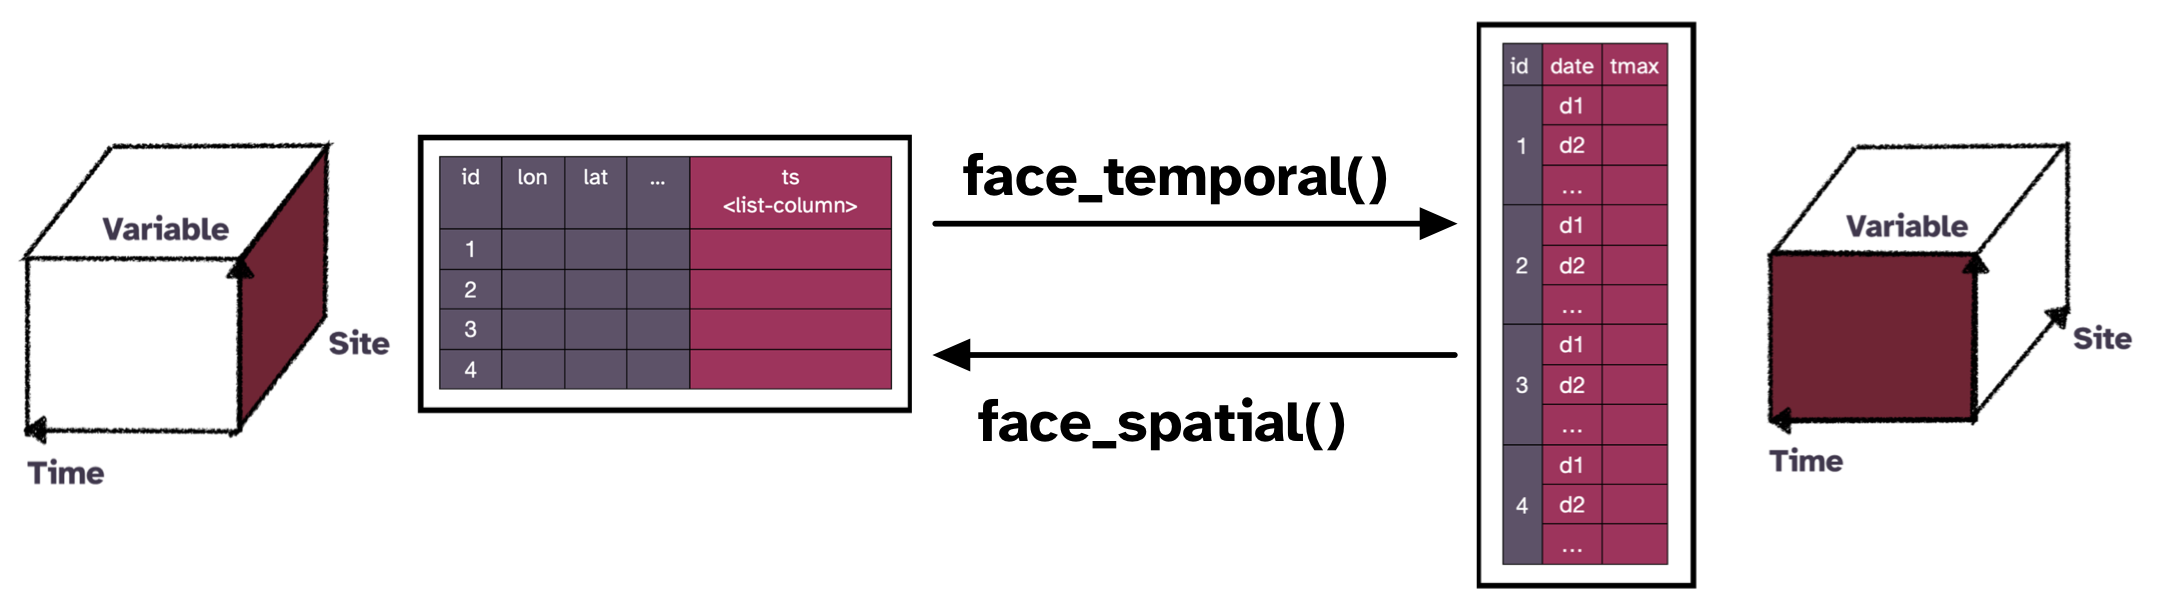
\includegraphics[width=1\linewidth]{figures/diagram-keynotes/diagram-keynotes.001} 

}

\caption{An illustration of the function \code{face\_temporal()} and \code{face\_spatial()}: \code{face\_temporal()} converts a spatial cubble (neseted form) into a temporal cubble (long form) to focus on the temporal variables. Conversely, \code{face\_spatial()} transforms a temporal cubble into a spatial one to emphasize spatial variables.}\label{fig:face}
\end{figure}
\end{CodeChunk}

\hypertarget{compatibility-with-tsibble-and-sf}{%
\subsection{Compatibility with tsibble and sf}\label{compatibility-with-tsibble-and-sf}}

Analysts often have their preferred spatial or temporal data structure that they prefer to use for spatio-temporal analysis. For example, the \code{tbl_ts} class from the \code{tsibble} package \citep{tsibble} is commonly used in time series forecasting and similarly, the \code{sf} class \citep{sf} is frequently used in spatial data science. In \code{cubble}, analysts have the flexibility to combine these two structures together by allowing the spatial component to also be an \code{sf} object and the temporal component to also be a \code{tsibble} object.

\hypertarget{using-a-tsibble-object-as-the-temporal-component}{%
\subsubsection{Using a tsibble object as the temporal component}\label{using-a-tsibble-object-as-the-temporal-component}}

The \code{key} and \code{index} arguments in a \code{cubble} object corresponds to the \code{tsibble} counterparts and they can be safely omitted, if the temporal component is a \code{tsibble} object, i.e.~\code{meteo_ts} in the example below. The \code{tsibble} class from the input will be carried over to the \code{cubble} object:

\begin{CodeChunk}
\begin{CodeInput}
R> ts_nested <- make_cubble(
+   spatial = stations, temporal = meteo_ts, coords = c(long, lat))
R> (ts_long <- face_temporal(ts_nested))
\end{CodeInput}
\begin{CodeOutput}
# cubble:   key: id [3], index: date, long form, [tsibble]
# temporal: 2020-01-01 -- 2020-01-10 [1D], no gaps
# spatial:  long [dbl], lat [dbl], elev [dbl], name [chr], wmo_id [dbl]
  id          date        prcp  tmax  tmin
  <chr>       <date>     <dbl> <dbl> <dbl>
1 ASN00086038 2020-01-01     0  26.8  11  
2 ASN00086038 2020-01-02     0  26.3  12.2
3 ASN00086038 2020-01-03     0  34.5  12.7
4 ASN00086038 2020-01-04     0  29.3  18.8
5 ASN00086038 2020-01-05    18  16.1  12.5
# i 25 more rows
\end{CodeOutput}
\begin{CodeInput}
R> class(ts_long)
\end{CodeInput}
\begin{CodeOutput}
[1] "temporal_cubble_df" "cubble_df"          "tbl_ts"            
[4] "tbl_df"             "tbl"                "data.frame"        
\end{CodeOutput}
\end{CodeChunk}

The temporal cubble shows \code{[tsibble]} in the header to indicate the object also being in a \code{tbl_ts} class (\code{tsibble}). Methods applies to the \code{tbl_ts} class can also be applied to the temporal cubble objects, for example, checking whether the data contain temporal gaps:

\begin{CodeChunk}
\begin{CodeInput}
R> ts_long |> has_gaps()
\end{CodeInput}
\begin{CodeOutput}
# A tibble: 3 x 2
  id          .gaps
  <chr>       <lgl>
1 ASN00086038 FALSE
2 ASN00086077 FALSE
3 ASN00086282 FALSE
\end{CodeOutput}
\end{CodeChunk}

An existing \code{cubble} object can promote its temporal component to a \code{tsibble} object by applying \code{make_temporal_tsibble()}. The following code illustrates this with the object \code{cb_long} created in section \ref{create} and the promoted cubble object is equal to the cubble object originally created from a \code{tsibble} object:

\begin{CodeChunk}
\begin{CodeInput}
R> ts_long2 <- cb_long |> make_temporal_tsibble() 
R> identical(ts_long2, ts_long)
\end{CodeInput}
\begin{CodeOutput}
[1] TRUE
\end{CodeOutput}
\end{CodeChunk}

\hypertarget{using-an-sf-object-as-the-spatial-component}{%
\subsubsection{Using an sf object as the spatial component}\label{using-an-sf-object-as-the-spatial-component}}

Similarly, an \code{sf} object can be supplied as the spatial component to create a \code{cubble} object, with the \code{coords} argument being omitted. This opens up the possibility to represent fixed area with polygons or multipolygons (see Applications \ref{covid}) and the \code{coords} argument will be calculated as the centroids of the (multi)polygons. The \code{[sf]} print in the cubble header suggest an spatial component being also a \code{sf} object:

\begin{CodeChunk}
\begin{CodeInput}
R> (sf_nested <- make_cubble(
+   spatial = stations_sf, temporal = meteo, 
+   key = id, index = date))
\end{CodeInput}
\begin{CodeOutput}
# cubble:   key: id [3], index: date, nested form, [sf]
# spatial:  [144.8321, -37.98, 145.0964, -37.6655], WGS 84
# temporal: date [date], prcp [dbl], tmax [dbl], tmin [dbl]
  id           elev name   wmo_id  long   lat            geometry ts      
  <chr>       <dbl> <chr>   <dbl> <dbl> <dbl>         <POINT [°]> <list>  
1 ASN00086038  78.4 essen~  95866  145. -37.7 (144.9066 -37.7276) <tibble>
2 ASN00086077  12.1 moora~  94870  145. -38.0   (145.0964 -37.98) <tibble>
3 ASN00086282 113.  melbo~  94866  145. -37.7 (144.8321 -37.6655) <tibble>
\end{CodeOutput}
\begin{CodeInput}
R> class(sf_nested)
\end{CodeInput}
\begin{CodeOutput}
[1] "spatial_cubble_df" "cubble_df"         "sf"               
[4] "tbl_df"            "tbl"               "data.frame"       
\end{CodeOutput}
\end{CodeChunk}

The \code{sf} functions applicable to a \code{cubble} object have been listed in Table \ref{tab:funs} and the following code shows how to perform coordinate transformation with \code{st_transform} on a cubble object:

\begin{CodeChunk}
\begin{CodeInput}
R> sf_nested |> sf::st_transform(crs = "EPSG:3857")
\end{CodeInput}
\begin{CodeOutput}
# cubble:   key: id [3], index: date, nested form, [sf]
# spatial:  [16122635.6225205, -4576600.8687746, 16152057.3639371,
#   -4532279.35567565], WGS 84
# temporal: date [date], prcp [dbl], tmax [dbl], tmin [dbl]
  id           elev name   wmo_id  long   lat            geometry ts      
  <chr>       <dbl> <chr>   <dbl> <dbl> <dbl>         <POINT [°]> <list>  
1 ASN00086038  78.4 essen~  95866  145. -37.7 (16130929 -4541016) <tibble>
2 ASN00086077  12.1 moora~  94870  145. -38.0 (16152057 -4576601) <tibble>
3 ASN00086282 113.  melbo~  94866  145. -37.7 (16122636 -4532279) <tibble>
\end{CodeOutput}
\end{CodeChunk}

The counterpart to promote the spatial component in an existing \code{cubble} to be an \code{sf} object is \code{make_spatial_sf()}:

\begin{CodeChunk}
\begin{CodeInput}
R> cb_nested |> make_spatial_sf() 
\end{CodeInput}
\begin{CodeOutput}
# cubble:   key: id [3], index: date, nested form, [sf]
# spatial:  [144.8321, -37.98, 145.0964, -37.6655], WGS 84
# temporal: date [date], prcp [dbl], tmax [dbl], tmin [dbl]
  id           long   lat  elev name   wmo_id ts                  geometry
  <chr>       <dbl> <dbl> <dbl> <chr>   <dbl> <list>           <POINT [°]>
1 ASN00086038  145. -37.7  78.4 essen~  95866 <tibble> (144.9066 -37.7276)
2 ASN00086077  145. -38.0  12.1 moora~  94870 <tibble>   (145.0964 -37.98)
3 ASN00086282  145. -37.7 113.  melbo~  94866 <tibble> (144.8321 -37.6655)
\end{CodeOutput}
\end{CodeChunk}

\hypertarget{tidyverse}{%
\subsection{Comparison to other spatio-temporal classes}\label{tidyverse}}

In \proglang{R}, there are other existing spatio-temporal data structure and this section compares and contrasts \pkg{cubble} with other existing alternative, specifically \pkg{stars} and \pkg{sftime}. The \pkg{stars} package \citep{stars} uses an array structure, as oppose to tibble, to represent multivariate spatio-temporal data. While both \pkg{stars} and \pkg{cubble} support vector and raster data, it is a matter of choice on which structure to use given the application. Analysts working on satellite imageries may prefer the array structure in \pkg{stars}, while others originally working with spatio-temporal data in 2D data frames may find \pkg{cubble} easier to adopt from their existing computing workflow.

The \pkg{sftime} package \citep{sftime} also builds from a tibble object and its focus is on handling irregular spatio-temporal data. This means \pkg{sftime} can also handle full space-time grids and sparse space-time layouts represented in \pkg{cubble}, but \pkg{cubble} uses nesting to avoid storing spatial variables repetitively at each timestamp. This provides memory efficiency when data is observed frequent, i.e.~daily or sub-daily, or the spatial geometry is expensive to repeat, i.e.~polygons or multipolygons. Consider the \code{climate_aus} data in the \pkg{cubble} package with 639 stations observed daily in a single year 2020. The created \code{sftime} object is approximately 14 times larger than the corresponding \code{cubble} object (118.24 MB vs.~8.52 MB).

\hypertarget{others}{%
\section{Other features and considerations}\label{others}}

\hypertarget{matching}{%
\subsection{Data fusion and matching}\label{matching}}

One common task when working with spatio-temporal data is to match nearby sites. For example, we may want to verify the location of an old list of stations with current stations, or we may want to match the data from different data sources. In cubble, spatial and temporal matching are performed using the functions \texttt{match\_spatial()} and \texttt{match\_temporal()}. The \texttt{match\_spatial()} function calculates the spatial distance between observations in two cubble objects. Various distance measures are available (check \texttt{sf::st\_distance}). Analysts can specify the number of matched groups to output using the \texttt{spatial\_n\_group} argument (default to 4 groups) and the number of matches per group using the \texttt{spatial\_n\_group} argument (default to 1, one-to-one matching). The syntax to use \texttt{match\_spatial()} is:

\begin{verbatim}
match_spatial(<cubble_obj1>, <cubble_obj2>, ...)
\end{verbatim}

The function \texttt{match\_temporal()} calculates the similarity between time series within spatially matched groups. Two identifiers are required: one for separating each matched group (\texttt{match\_id}) and one for separating the two data sources (\texttt{data\_id}). The argument \texttt{temporal\_by} uses the \texttt{by} syntax from dplyr's \texttt{*\_join} to specify the temporal variables to match.

The similarity score between two time series is calculated using a matching function, which can be customised by the analysts. The matching function takes two time series as a list and returns a single numerical score. This allows for flexibility in using existing time series distance calculation implementation. By default, cubble implements a simple peak matching algorithm (\texttt{match\_peak}) that counts the number of peaks in two time series that fall within a specified temporal window. The syntax to use \texttt{match\_temporal()} is

\begin{verbatim}
match_temporal(
  <cubble_obj_from_match_spatial>, 
  data_id = , match_id = , 
  temporal_by = c("..." = "...")
)
\end{verbatim}

\hypertarget{interactive-graphics}{%
\subsection{Interactive graphics}\label{interactive-graphics}}

The workflow with the \code{cubble} class works well with an interactive graphics pipeline (e.g., \citet{buja1988elements}; \citet{buja1996interactive}; \citet{sutherland2000orca}; \citet{xie2014reactive}; \citet{cheng2016enabling}) that is available in \proglang{R} with the package \pkg{crosstalk} \citep{crosstalk}. Figure \ref{fig:illu-interactive} illustrates the linking between a map and multiple time series in a \code{cubble} object. Both the map, generated from the spatial cubble, and the time series plot, generated from the temporal cubble, are shared crosstalk objects. When a user selects a location on the map (a), the corresponding site is highlighted. This selection activates a row in the spatial \code{cubble}, which is then communicated to the temporal \code{cubble}, resulting in the selection of all observations with the same ID in (b). Consequently the temporal \code{cubble} highlights the corresponding series in the time series plot (c). Linking can also be initiated from the time series plot, by selecting points on the time series. This action activates rows with the same ID in the temporal \code{cubble} and the row in the spatial \code{cubble}, which will be highlighted on the map. Please refer to the appendix for the corresponding illustration.

\begin{CodeChunk}
\begin{figure}

{\centering 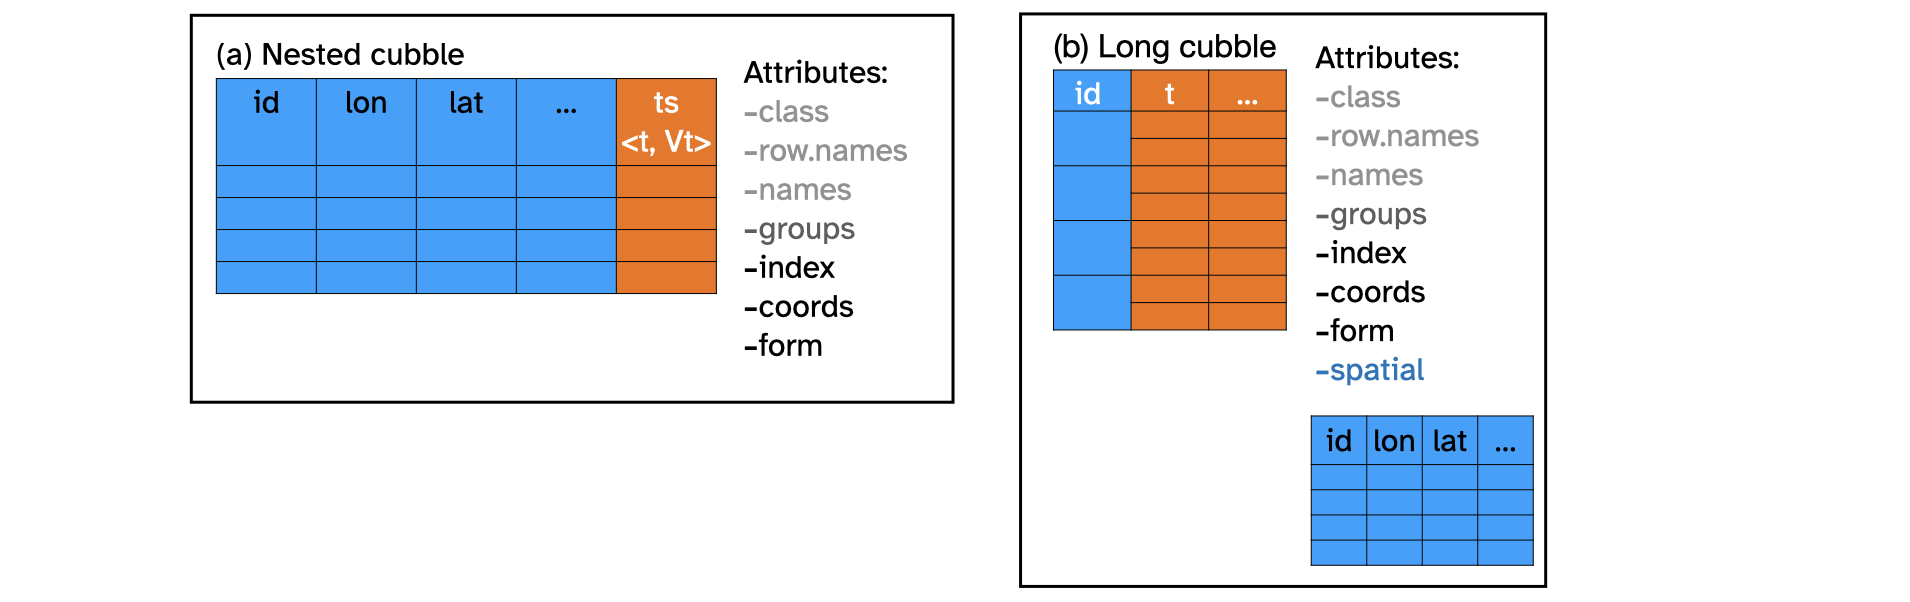
\includegraphics[width=1\linewidth,height=0.35\textheight]{figures/diagram-keynotes/diagram-keynotes.002} 

}

\caption{Linking between multiple plots. The line plots and the map are constructed from shared \code{crosstalk} objects. When a station is selected on the map (a), the corresponding row in the spatial \code{cubble} will be activated. This will link to all the rows with the same id in the temporal \code{cubble} (b) and update the line plot (c).}\label{fig:illu-interactive}
\end{figure}
\end{CodeChunk}

\hypertarget{st_transformation}{%
\subsection{Spatio-temporal transformations}\label{st_transformation}}

Sometimes, we wish to communicate spatial and temporal information collectively through visualisation. This can be achieved through several graphical displays: one can make faceted maps across time, creating map animations, or constructing interactive graphics to link between map and time series plot. The concept of glyph maps was initially proposed in \citet{Wickham2012-yr}. The underlying idea is to transform the temporal coordinates into spatial coordinates so that time series plot can be displayed on the map.

The package \texttt{GGally} initially implement the glyph map. It uses \texttt{glyphs()} to calculate the axis transformation and then uses \texttt{geom\_polygon()} to draw the map. In cubble, a ggproto implementation \texttt{geom\_glyph()} performs the linear algebra internally as data transformation . The \texttt{geom\_glyph()} requires four aesthetics: \texttt{x\_major}, \texttt{y\_major}, \texttt{x\_minor}, and \texttt{y\_minor}. The major axes are the outer spatial coordinates and the minor axes are the inner/ temporal coordinates:

\begin{verbatim}
data |> 
  ggplot() +
  geom_glyph(aes(x_major = ..., x_minor = ..., 
                 y_major = ..., y_minor = ...))
\end{verbatim}

Some useful controls over the glyph map includes:

\begin{itemize}
\tightlist
\item
  polar coordinate glyph maps with \code{polar = TRUE},
\item
  adjust glyph size with arguments \code{width} and \code{height},
\item
  glyph scale to fixed (\code{global_rescale} defaults to \code{TRUE}) or free, and
\item
  reference boxes and lines with \code{geom_glyph_box()} and \code{geom_glyph_line()}.
\end{itemize}

\hypertarget{examples}{%
\section{Applications}\label{examples}}

Five examples are chosen to illustrate different aspects of the \pkg{cubble} package: creating a \code{cubble} object from two Coronavirus (COVID) data tables with the complication of differing location names, using spatial transformations to make a glyph map of seasonal temperature changes, matching river level data and weather station records for analysis of water supply, reading NetCDF format data to reproduce a climate reanalysis plot, and the workflow to create complex interactive linked plots.

\hypertarget{covid}{%
\subsection{Victoria COVID spatio-temporal incidence and spread}\label{covid}}

Since the start of the pandemic, the Victoria State Government in Australia has been providing daily COVID counts per Local Government Area (LGA). This data can be combined with map polygon data, available from the Australian Bureau of Statistics (ABS), to visualize COVID incidence and spread. In the \pkg{cubble} package, the COVID count data (\code{covid}) and the LGA information (\code{lga}) are available as a \code{tsibble} object and an \code{sf} object respectively.

A cubble object can be created from separate spatial and temporal component using the \code{make_cubble()} function, introduced in Section \ref{create}. The \code{by} argument
is used to specify the joining variable from the two component using the \code{*_join()} \code{by} syntax:

\begin{CodeChunk}
\begin{CodeInput}
R> cb <- make_cubble(lga, covid, by = c("lga_name_2018" = "lga"))
\end{CodeInput}
\begin{CodeOutput}
Warning: st_centroid assumes attributes are constant over geometries
\end{CodeOutput}
\begin{CodeOutput}
! Some sites in the spatial table don't have temporal information
\end{CodeOutput}
\begin{CodeOutput}
! Some sites in the temporal table don't have spatial information
\end{CodeOutput}
\begin{CodeOutput}
! Use `check_key()` to check on the unmatched key
The cubble is created only with sites having both spatial and
temporal information
\end{CodeOutput}
\end{CodeChunk}

The warning message suggests the slight difference of LGA encoding used by Victoria government and ABS and prompts analysts to use the function \code{check_key()} to identify the mismatches:

\begin{CodeChunk}
\begin{CodeInput}
R> (check_res <- check_key(
+   spatial = lga, temporal = covid, 
+   by = c("lga_name_2018" = "lga")
+ ))
\end{CodeInput}
\begin{CodeOutput}
$paired
# A tibble: 78 x 2
  spatial        temporal      
  <chr>          <chr>         
1 Alpine (S)     Alpine (S)    
2 Ararat (RC)    Ararat (RC)   
3 Ballarat (C)   Ballarat (C)  
4 Banyule (C)    Banyule (C)   
5 Bass Coast (S) Bass Coast (S)
# i 73 more rows

$potential_pairs
# A tibble: 2 x 2
  spatial             temporal    
  <chr>               <chr>       
1 Kingston (C) (Vic.) Kingston (C)
2 Latrobe (C) (Vic.)  Latrobe (C) 

$others
$others$spatial
character(0)

$others$temporal
[1] "Interstate" "Overseas"   "Unknown"   
\end{CodeOutput}
\end{CodeChunk}

The result of the \code{check_key()} function is a list containing three elements: 1) matched keys from both tables, 2) potentially paired keys, and 3) others. Here, the main mismatch arises from the two LGAs: Kingston and Latrobe (Kingston is a LGA in both Victoria and South Australia and Latrobe is a LGA in both Victoria and Tasmania). Analysts can modify the input spatial and temporal data accordingly and recreate the cubble object:

\begin{CodeChunk}
\begin{CodeInput}
R> lga2 <- lga |>
+   rename(lga = lga_name_2018) |> 
+   mutate(lga = ifelse(lga == "Kingston (C) (Vic.)", "Kingston (C)", lga),
+          lga = ifelse(lga == "Latrobe (C) (Vic.)", "Latrobe (C)", lga))
R>   
R> covid2 <- covid |> filter(!lga %in% check_res$others$temporal)
R> 
R> (cb <- make_cubble(spatial = lga2, temporal = covid2))
\end{CodeInput}
\begin{CodeOutput}
# cubble:   key: lga [80], index: date, nested form, [sf]
# spatial:  [140.961682, -39.1339581, 149.976291, -33.9960517], WGS 84
# temporal: date [date], n [dbl], avg_7day [dbl]
  lga             long   lat                                   geometry ts      
  <chr>          <dbl> <dbl>                             <GEOMETRY [°]> <list>  
1 Alpine (S)      147. -36.9 POLYGON ((146.7258 -36.45922, 146.7198 -3~ <tbl_ts>
2 Ararat (RC)     143. -37.5 POLYGON ((143.1807 -37.73152, 143.0609 -3~ <tbl_ts>
3 Ballarat (C)    144. -37.5 POLYGON ((143.6622 -37.57241, 143.68 -37.~ <tbl_ts>
4 Banyule (C)     145. -37.7 POLYGON ((145.1357 -37.74091, 145.1437 -3~ <tbl_ts>
5 Bass Coast (S)  146. -38.5 MULTIPOLYGON (((145.5207 -38.30667, 145.5~ <tbl_ts>
# i 75 more rows
\end{CodeOutput}
\end{CodeChunk}

\hypertarget{historicaltmax}{%
\subsection{Australian historical maximum temperature}\label{historicaltmax}}

The Global Historical Climatology Network (GHCN) provides daily climate measures for stations worldwide. In the \pkg{cubble} package, the dataset \code{historical_tmax} contains daily maximum temperature data for 75 stations in Australia, covering two periods: 1971-1975 and 2016-2020. The objective of this example is to compare the changes in maximum temperature between these two periods using a glyph map.

To prevent overlapping of weather stations on the map, we subset the stations based on minimum distance of 50km between them. This can be done by first promoting the spatial cubble to also be an sf object with \code{make_spatial_sf()}, calculating the distance matrix using the sf function \code{st_distance()}, and filtering the stations with dplyr's \code{filter()}:

\begin{CodeChunk}
\begin{CodeInput}
R> a <- historical_tmax |> make_spatial_sf() |> st_distance()
R> a[upper.tri(a, diag = TRUE)] <- 1e6
R> 
R> (tmax <- historical_tmax |> 
+   filter(rowSums(a < units::as_units(50, "km")) == 0))
\end{CodeInput}
\begin{CodeOutput}
# cubble:   key: id [54], index: date, nested form
# spatial:  [141.2652, -39.1297, 153.3633, -28.9786], Missing CRS!
# temporal: date [date], tmax [dbl]
  id           long   lat  elev name                     wmo_id ts      
  <chr>       <dbl> <dbl> <dbl> <chr>                     <dbl> <list>  
1 ASN00047016  141. -34.0    43 lake victoria storage     94692 <tibble>
2 ASN00047019  142. -32.4    61 menindee post office      94694 <tibble>
3 ASN00048015  147. -30.0   115 brewarrina hospital       95512 <tibble>
4 ASN00048027  146. -31.5   260 cobar mo                  94711 <tibble>
5 ASN00048031  149. -29.5   145 collarenebri (albert st)  95520 <tibble>
# i 49 more rows
\end{CodeOutput}
\end{CodeChunk}

Next, daily maximum temperature is averaged into monthly series for each periods in the temporal cubble. The last step with \code{unfold()} moves the two coordinate columns \code{long, lat} into the temporal cubble, preparing the data for the glyph map:

\begin{CodeChunk}
\begin{CodeInput}
R> (tmax <- tmax |>
+   face_temporal() |> 
+   group_by(
+     yearmonth = tsibble::make_yearmonth(
+       year = ifelse(lubridate::year(date) > 2015, 2016, 1971),
+       month = lubridate::month(date))
+   )|>
+   summarise(tmax = mean(tmax, na.rm = TRUE)) |> 
+   mutate(group = as.factor(lubridate::year(yearmonth)),
+          month = lubridate::month(yearmonth)) |> 
+   unfold(long, lat))
\end{CodeInput}
\begin{CodeOutput}
# cubble:   key: id [54], index: yearmonth, long form
# temporal: 1971 Jan -- 2016 Dec [1M], has gaps!
# spatial:  long [dbl], lat [dbl], elev [dbl], name [chr], wmo_id [dbl]
  yearmonth id           tmax group month  long   lat
      <mth> <chr>       <dbl> <fct> <dbl> <dbl> <dbl>
1  1971 Jan ASN00047016  31.1 1971      1  141. -34.0
2  1971 Jan ASN00047019  33.1 1971      1  142. -32.4
3  1971 Jan ASN00048015  33.9 1971      1  147. -30.0
4  1971 Jan ASN00048027  32.5 1971      1  146. -31.5
5  1971 Jan ASN00048031  33.3 1971      1  149. -29.5
# i 1,276 more rows
\end{CodeOutput}
\end{CodeChunk}

A quick check on the number of observations for each location is made, revealing that there are several with less than 24 observations -- these stations lack temperature values for some months. In this example, those stations are removed by switching to the spatial \code{cubble} to operate on the spatial component over time, and then, move back into the temporal \code{cubble} (to make the glyph map):

\begin{CodeChunk}
\begin{CodeInput}
R> tmax <- tmax |> 
+   face_spatial() |> 
+   rowwise() |>
+   filter(nrow(ts) == 24) |>
+   face_temporal()
\end{CodeInput}
\end{CodeChunk}

The following code creates the glyph map (a) in Figure \ref{fig:glyphmap} with additional ggplot2 code for highlighting the single station, Cobar and styling:

\begin{verbatim}
nsw_vic <- ozmaps::abs_ste |> 
  filter(NAME %in% c("Victoria","New South Wales"))

tmax |> 
  ggplot(aes(x_major = long, x_minor = month, 
             y_major = lat, y_minor = tmax,
             group = interaction(id, group))) + 
  geom_sf(data =  nsw_vic, ...,  inherit.aes = FALSE) + 
  geom_glyph_box(width = 0.8, height = 0.3) + 
  geom_glyph(aes(color = group), width = 0.8, height = 0.3) +
  ...
\end{verbatim}

\begin{CodeChunk}
\begin{figure}

{\centering 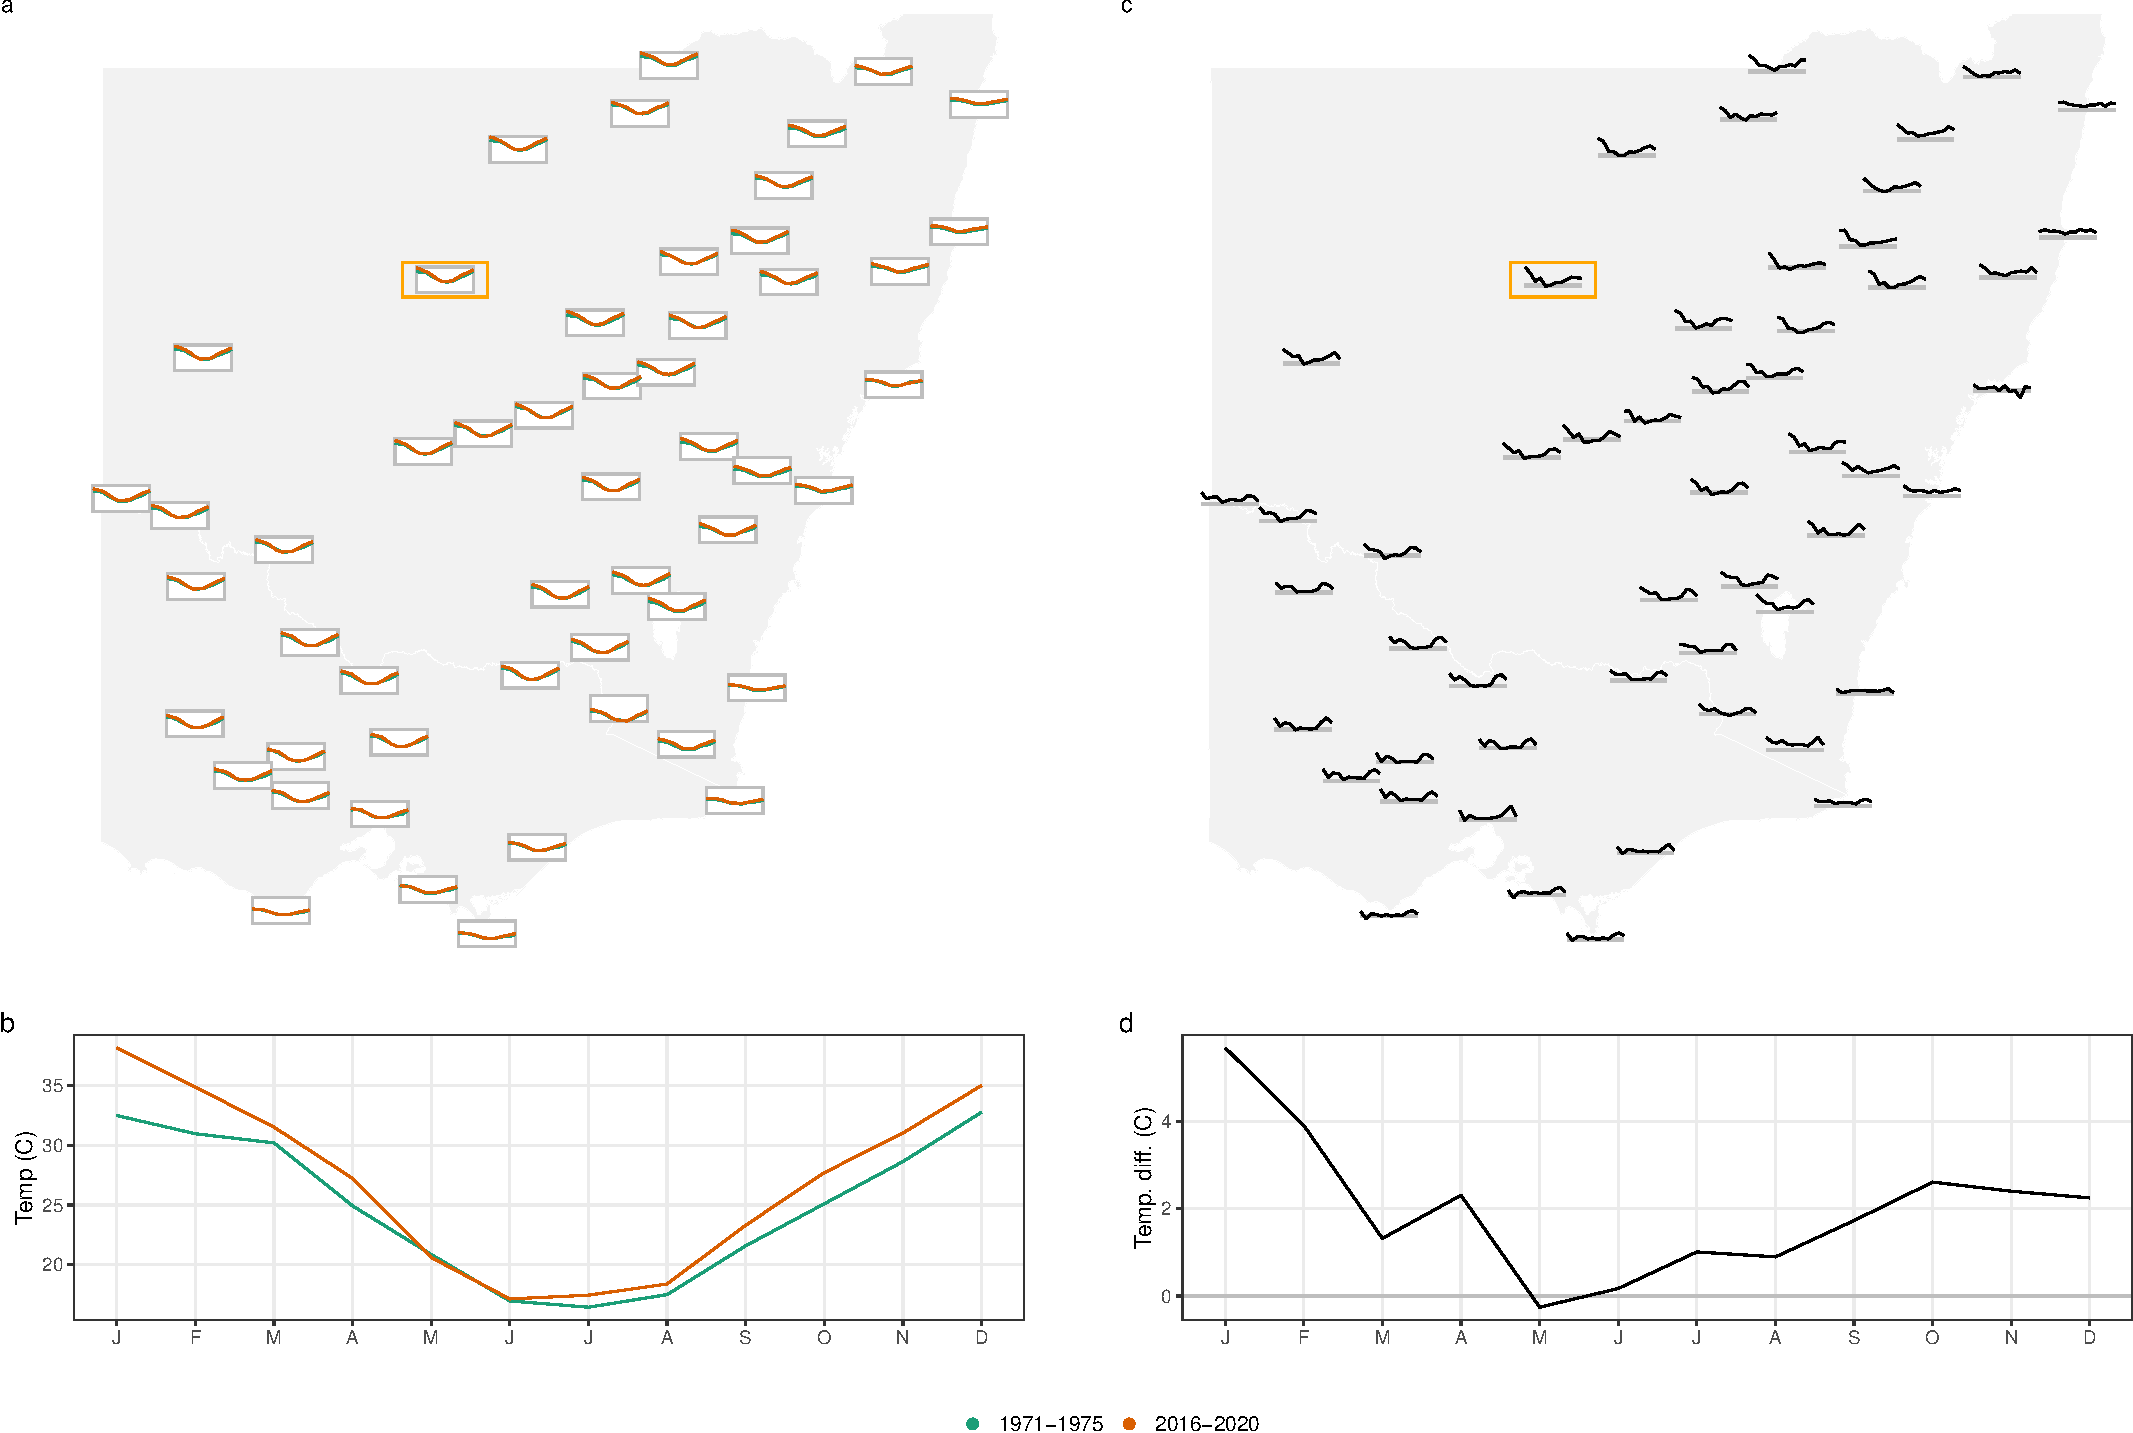
\includegraphics[width=1\linewidth]{/Users/hzha400/Documents/research/paper-cubble/figures/glyphmap-1} 

}

\caption[Comparison of average maximum temperature between 1971-1975 and 2016-2020 for 54 stations in Victoria and New South Wales, Australia]{Comparison of average maximum temperature between 1971-1975 and 2016-2020 for 54 stations in Victoria and New South Wales, Australia. (a) and (b): the monthly temperature series for the two periods in a glyph map and for a single station Cobar, highlighted in orange in the glyph map. (c) and (d): the difference series between the two periods (2016s minus 1971s) in a glyph map and for station Cobar. The grey horizontal line marks zero difference. The glyph map displaying the difference series (c) reveals more pronounced changes between the two periods, with many inland locations in New South Wales show an increased temperature in late summer (Jan-Feb) in recent years.}\label{fig:glyphmap}
\end{figure}
\end{CodeChunk}

\hypertarget{river-levels-and-rainfall-in-victoria}{%
\subsection{River levels and rainfall in Victoria}\label{river-levels-and-rainfall-in-victoria}}

One common task when working with spatio-temporal data is to match nearby sites. For example, we may want to verify the location of an old list of stations with current stations, or we may want to match the data from different data sources. In this example, we will introduce the spatial and temporal matching in cubble using an example on matching river level data with precipitation in Victoria, Australia.

The water level data collected by the Bureau of Meteorology, can be compared with the precipitation since rainfall can directly impact water level in river. Both \texttt{climate\_vic} and \texttt{river} are cubble objects, and we can obtain a summary of the 10 closest pairs between them:

\begin{CodeChunk}
\begin{CodeInput}
R> res_sp <- match_spatial(climate_vic, river, spatial_n_group = 10)
R> print(res_sp, n = 20)
\end{CodeInput}
\begin{CodeOutput}
# A tibble: 10 x 4
   from        to      dist group
   <chr>       <chr>    [m] <int>
 1 ASN00088051 406213 1838.     1
 2 ASN00084145 222201 2185.     2
 3 ASN00085072 226027 3282.     3
 4 ASN00080015 406704 4034.     4
 5 ASN00085298 226027 4207.     5
 6 ASN00082042 405234 6153.     6
 7 ASN00086038 230200 6167.     7
 8 ASN00086282 230200 6928.     8
 9 ASN00085279 224217 7431.     9
10 ASN00080091 406756 7460.    10
\end{CodeOutput}
\end{CodeChunk}

The result can also be returned as cubble objects by setting the argument \texttt{return\_cubble\ =\ TRUE}. The output is be a list where each element is a paired cubble object. To combine all the results into a single cubble, you can use \texttt{bind\_rows()}. In the case when a site in the second cubble (the \texttt{river} data here) is matched to two stations in the first cubble (\texttt{climate\_vic} here), the binding may not be successful since cubble requires unique rows in the nested form. In the summary table above, the river station \texttt{226027} is matched to more than one weather station: \texttt{ASN00085072} (group 3) and \texttt{ASN00085298} (group 5). Similarly, the river station \texttt{230200} is matched in group 7 and 8). In such cases, you can either deselect one pair before combining, or work with the list output with the \texttt{purrr::map} syntax:

\begin{CodeChunk}
\begin{CodeInput}
R> res_sp <- match_spatial(
+   climate_vic, river, 
+   spatial_n_group = 10, return_cubble = TRUE)
R> str(res_sp, max.level = 0)
\end{CodeInput}
\begin{CodeOutput}
List of 10
\end{CodeOutput}
\begin{CodeInput}
R> (res_sp <- res_sp[-c(5, 8)] |> bind_rows())
\end{CodeInput}
\begin{CodeOutput}
# cubble:   key: id [16], index: date, nested form, [sf]
# spatial:  [144.5203, -38.144913, 148.4667, -36.128657], WGS 84
# temporal: date [date], prcp [dbl], tmax [dbl], tmin [dbl]
  id      long   lat  elev name  wmo_id ts       type              geometry
  <chr>  <dbl> <dbl> <dbl> <chr>  <dbl> <list>   <chr>          <POINT [°]>
1 ASN00~  145. -37.0 290   rede~  94859 <tibble> clim~  (144.5203 -37.0194)
2 406213  145. -37.0  NA   CAMP~     NA <tibble> river (144.5403 -37.01512)
3 ASN00~  148. -37.7  62.7 orbo~  95918 <tibble> clim~  (148.4667 -37.6922)
4 222201  148. -37.7  NA   SNOW~     NA <tibble> river  (148.451 -37.70739)
5 ASN00~  147. -38.1   4.6 east~  94907 <tibble> clim~  (147.1322 -38.1156)
# i 11 more rows
# i 2 more variables: group <int>, dist [m]
\end{CodeOutput}
\end{CodeChunk}

For temporal matching, we match the variable \texttt{Water\_course\_level} from the river data to \texttt{prcp} in the weather station data. The variable \texttt{group} and \texttt{types} identify the matching group and the two datasets:

\begin{CodeChunk}
\begin{CodeInput}
R> (res_tm <- res_sp |> 
+   match_temporal(
+     data_id = type, match_id = group,
+     temporal_by = c("prcp" = "Water_course_level")))
\end{CodeInput}
\begin{CodeOutput}
# A tibble: 8 x 2
  group match_res
  <int>     <dbl>
1     1        30
2     2         5
3     3        14
4     4        20
5     6        23
# i 3 more rows
\end{CodeOutput}
\end{CodeChunk}

Similarly, the cubble output can be returned using the argument \texttt{return\_cubble\ =\ TRUE}. Here we select the four pairs with the highest number of matching peaks:

\begin{CodeChunk}
\begin{CodeInput}
R> res_tm <- res_sp |> 
+   match_temporal(
+     data_id = type, match_id = group,
+     temporal_by = c("prcp" = "Water_course_level"),
+     return_cubble = TRUE)
R> (res_tm <- res_tm |> bind_rows() |> filter(group %in% c(1, 7, 6, 9)))
\end{CodeInput}
\begin{CodeOutput}
# cubble:   key: id [8], index: date, nested form, [sf]
# spatial:  [144.5203, -37.8817, 147.572223, -36.8472], WGS 84
# temporal: date [date], matched [dbl]
  id         long   lat  elev name  wmo_id type              geometry group
  <chr>     <dbl> <dbl> <dbl> <chr>  <dbl> <chr>          <POINT [°]> <int>
1 ASN00088~  145. -37.0 290   rede~  94859 clim~  (144.5203 -37.0194)     1
2 406213     145. -37.0  NA   CAMP~     NA river (144.5403 -37.01512)     1
3 ASN00082~  146. -36.8 502   stra~  95843 clim~  (145.7308 -36.8472)     6
4 405234     146. -36.9  NA   SEVE~     NA river (145.6828 -36.88701)     6
5 ASN00086~  145. -37.7  78.4 esse~  95866 clim~  (144.9066 -37.7276)     7
# i 3 more rows
# i 3 more variables: dist [m], ts <list>, match_res <dbl>
\end{CodeOutput}
\end{CodeChunk}

Figure \ref{fig:matching} shows four matched pairs on the map (a) and standardized data as time series (b) with concurrent increasing.

\begin{CodeChunk}
\begin{figure}

{\centering 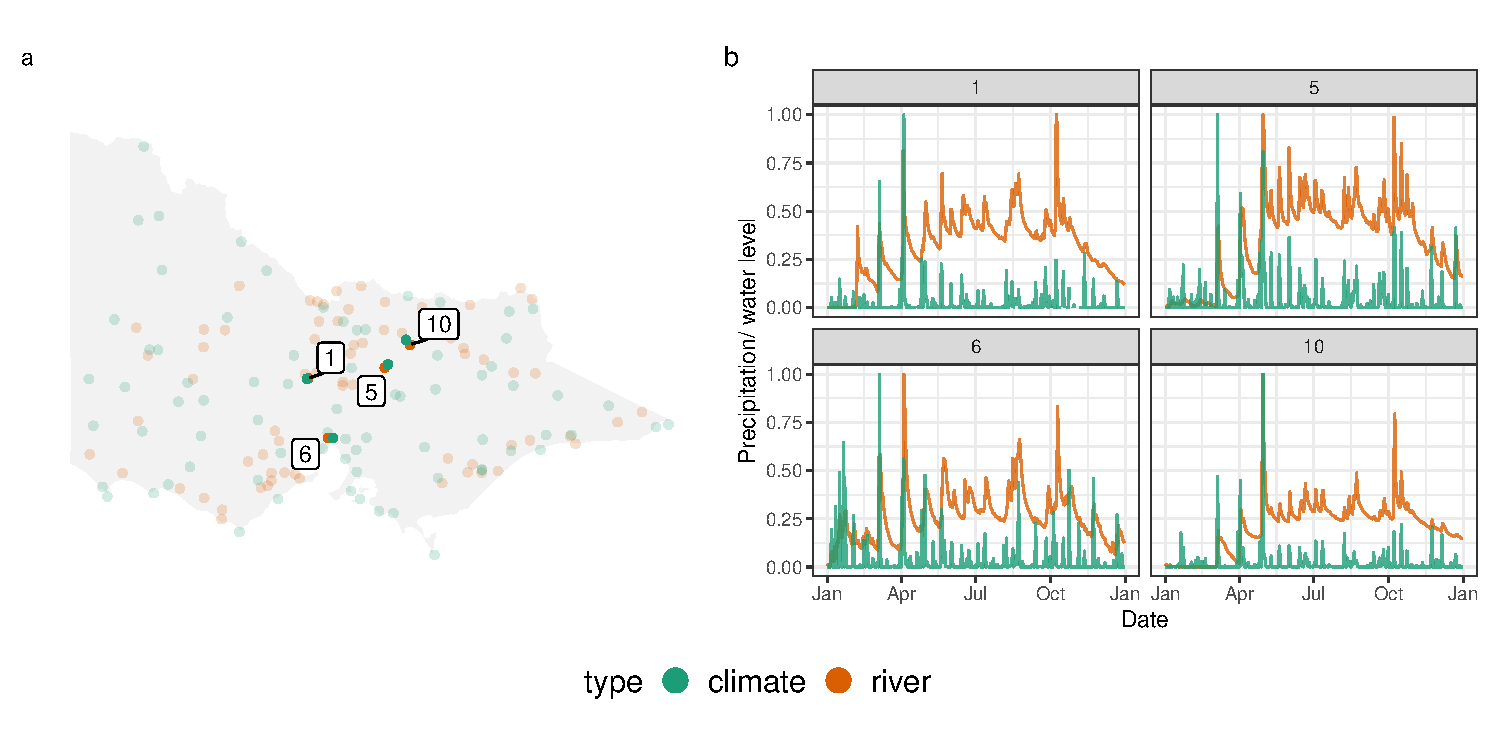
\includegraphics[width=1\linewidth]{/Users/hzha400/Documents/research/paper-cubble/figures/matching-1} 

}

\caption[Weather stations and river gauges with matched pairs labelled on the map (a) and plotted across time (b)]{Weather stations and river gauges with matched pairs labelled on the map (a) and plotted across time (b). Precipitation and water level have been standardised between 0 and 1 to be displayed on the same scale. The water level reflects the increase in precipitation. The numbers (1, 7, 6, 9) indicate the group index derived from spatial matching, only those that were selectd by temporal matching are shown here.}\label{fig:matching}
\end{figure}
\end{CodeChunk}

\hypertarget{era5-climate-reanalysis-data}{%
\subsection{ERA5: climate reanalysis data}\label{era5-climate-reanalysis-data}}

The ERA5 reanalysis \citep{hersbach2020era5} provides hourly estimates of atmospheric, land and oceanic climate variables on a global scale. The hourly pressure level data in the NetCDF format can be downloaded from Copernicus Climate Data Store (CDS) \citep{cds} or via the \pkg{ecmwfr} package \citep{ecwmfr}. This example reproduces the row created from ERA5 reanalysis data shown in Figure 19 by \citet{hersbach2020era5}. The plot shows the southern polar vortex splitting into two on 2002-09-26, and further splitting into four on 2002-10-04. Further explanation of why this is interesting can be found in the figure source, and also in \citet{simmons2020global} and \citet{simmons2005ecmwf}.

To work with NetCDF data in R, several packages are available, including \code{ncdf4}, \code{RNetCDF}, and \code{tidync}. The following code converts a NetCDF object of class \code{ncdf4} into a cubble object:

\begin{CodeChunk}
\begin{CodeInput}
R> raw <- ncdf4::nc_open(here::here("data/era5-pressure.nc"))
\end{CodeInput}
\end{CodeChunk}

Analysts can extract a subset of the NetCDF data with the arguments \code{vars}, \code{long_range} and \code{lat_range}. In this example, the variables q (specific humidity) and z (geopotential) are selected and the coordinates are subsetted to every degree in longitude and latitude:

\begin{CodeChunk}
\begin{CodeInput}
R> (dt <- as_cubble(raw, vars = c("q", "z"),
+                  long_range = seq(-180, 180, 1), lat_range = seq(-88, -15, 1)))
\end{CodeInput}
\begin{CodeOutput}
# cubble:   key: id [26640], index: time, nested form
# spatial:  [-180, -88, 179, -15], Missing CRS!
# temporal: time [date], q [dbl], z [dbl]
     id  long   lat ts              
  <int> <dbl> <dbl> <list>          
1     1  -180   -15 <tibble [8 x 3]>
2     2  -179   -15 <tibble [8 x 3]>
3     3  -178   -15 <tibble [8 x 3]>
4     4  -177   -15 <tibble [8 x 3]>
5     5  -176   -15 <tibble [8 x 3]>
# i 26,635 more rows
\end{CodeOutput}
\end{CodeChunk}

Once the NetCDF data is coerced into a cubble object, subsequent analysis can be conducted to filter on the date of interest, scale the variable specific humidity and create visualisation in ggplot as in Figure \ref{fig:netcdf}.

\begin{CodeChunk}
\begin{figure}

{\centering 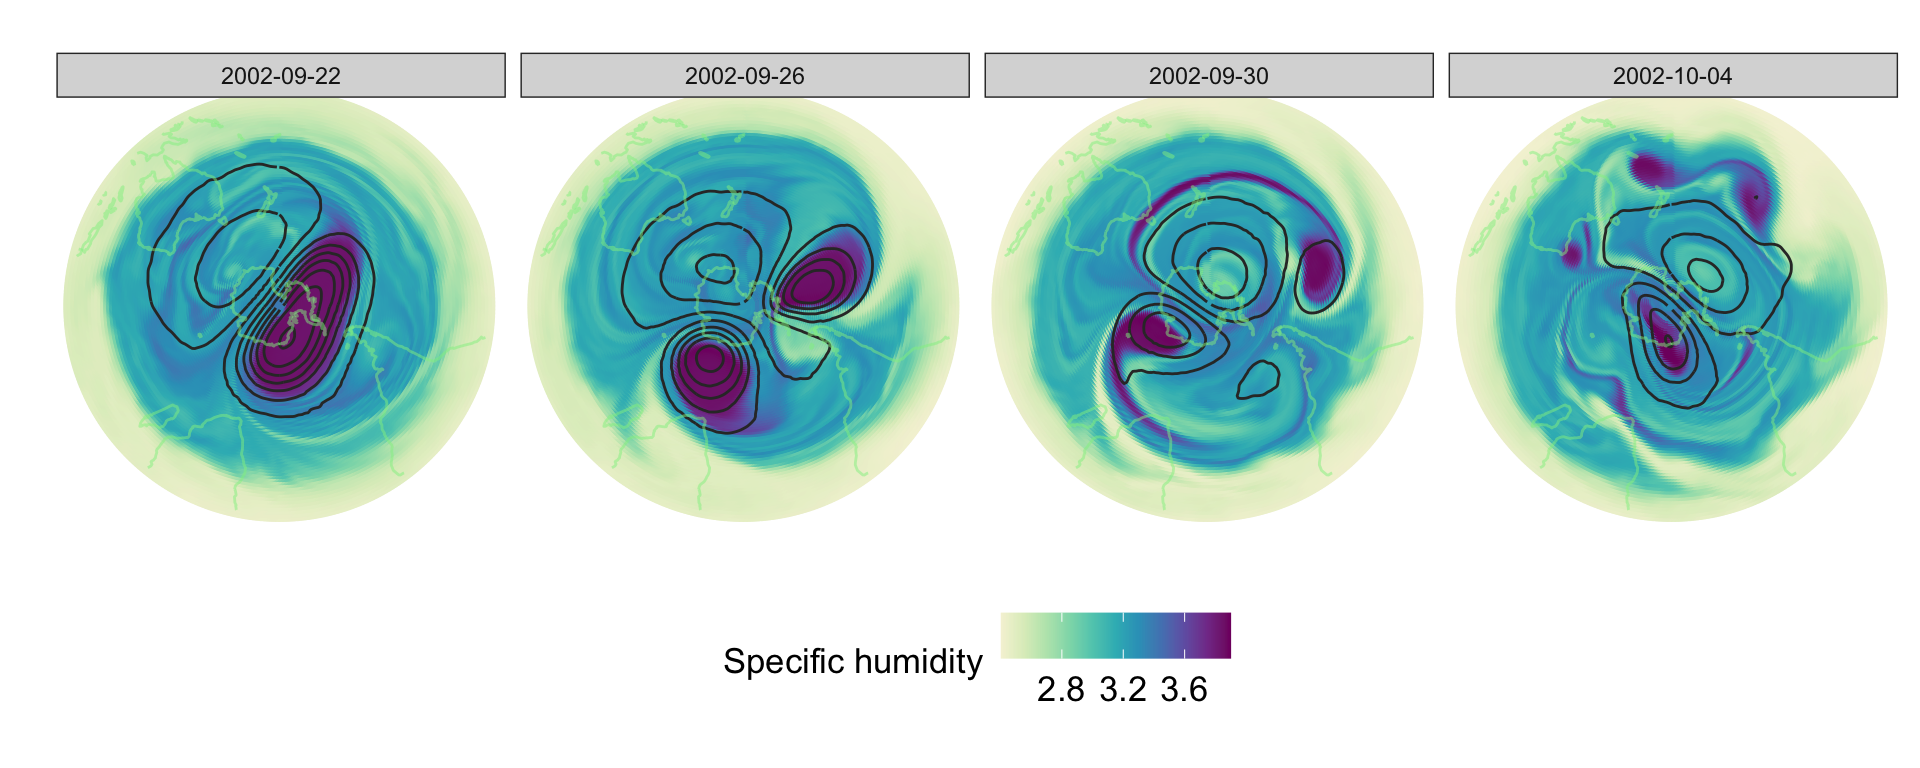
\includegraphics[width=1\linewidth]{/Users/hzha400/Documents/research/paper-cubble/figures/netcdf-1} 

}

\caption[A reproduction of the second row (ERA5 data) of Figure 19 in Hersbach et al (2020) to illustrate the break-up of sourthern polar vortex in late September and early October 2002]{A reproduction of the second row (ERA5 data) of Figure 19 in Hersbach et al (2020) to illustrate the break-up of sourthern polar vortex in late September and early October 2002. The polar vortex, signalled by the high specific humidity, splits into two on 2002-09-26 and further splits into four on 2002-10-04.}\label{fig:netcdf}
\end{figure}
\end{CodeChunk}

\hypertarget{australian-temperature-range}{%
\subsection{Australian temperature range}\label{australian-temperature-range}}

Interactive graphics can be useful because they make it possible to look at the data in multiple ways on-the-fly. This is especially important for spatio-temporal data, where we would like to interactively connect spatial and temporal displays. This example describes the process of using the \pkg{cubble} package with the \pkg{crosstalk} package to build an interactive display connecting a map of Australia, with ribbon plots of temperature range observed at the stations. The purpose is to explore the variation of monthly temperature range over the country. Figure \ref{fig:interactive-linking} shows three snapshots of the interactivity.

The key steps are to convert both the nested and long forms of the data into shared \code{crosstalk} objects, and to plot these side-by-side. The two are linked by the station identifier.

\begin{Shaded}
\begin{Highlighting}[]
\NormalTok{clean }\OtherTok{\textless{}{-}}\NormalTok{ climate\_full }\SpecialCharTok{|\textgreater{}}\NormalTok{ ...}

\NormalTok{nested }\OtherTok{\textless{}{-}}\NormalTok{ clean }\SpecialCharTok{|\textgreater{}}\NormalTok{ SharedData}\SpecialCharTok{$}\FunctionTok{new}\NormalTok{(}\SpecialCharTok{\textasciitilde{}}\NormalTok{id, }\AttributeTok{group =} \StringTok{"cubble"}\NormalTok{)}
\NormalTok{long }\OtherTok{\textless{}{-}} \FunctionTok{face\_temporal}\NormalTok{(clean) }\SpecialCharTok{|\textgreater{}}\NormalTok{ SharedData}\SpecialCharTok{$}\FunctionTok{new}\NormalTok{(}\SpecialCharTok{\textasciitilde{}}\NormalTok{id, }\AttributeTok{group =} \StringTok{"cubble"}\NormalTok{)}

\NormalTok{p1 }\OtherTok{\textless{}{-}}\NormalTok{ nested }\SpecialCharTok{|\textgreater{}}\NormalTok{ ...}
\NormalTok{p2 }\OtherTok{\textless{}{-}}\NormalTok{ long }\SpecialCharTok{|\textgreater{}}\NormalTok{ ...}

\NormalTok{crosstalk}\SpecialCharTok{::}\FunctionTok{bscols}\NormalTok{(plotly}\SpecialCharTok{::}\FunctionTok{ggplotly}\NormalTok{(p1), plotly}\SpecialCharTok{::}\FunctionTok{ggplotly}\NormalTok{(p2), ...)}
\end{Highlighting}
\end{Shaded}

Plot (a) shows the initial state of the interactive display: all locations are shown as dots on the map, coloured by temperature range, and the right plot shows the ribbons representing maximum to minimum for all stations. In plot (b) the ``Mount Elizabeth'' station, which shows a high variance colour on the initial map, is selected on the map and this produces the ribbon on the right. In plot (c) the lowest temperature in August is selected, which is ``Thredbo'' station on the left map. It was surprising to us that this was not a station in Tasmania, so for comparison a station in Tasmania is selected on the map to show in relation to Thredbo. We can see that Thredbo has a bigger winter dip in temperature, and although Tasmania is cold generally, it's temperatures are more constant

\begin{CodeChunk}
\begin{figure}

{\centering 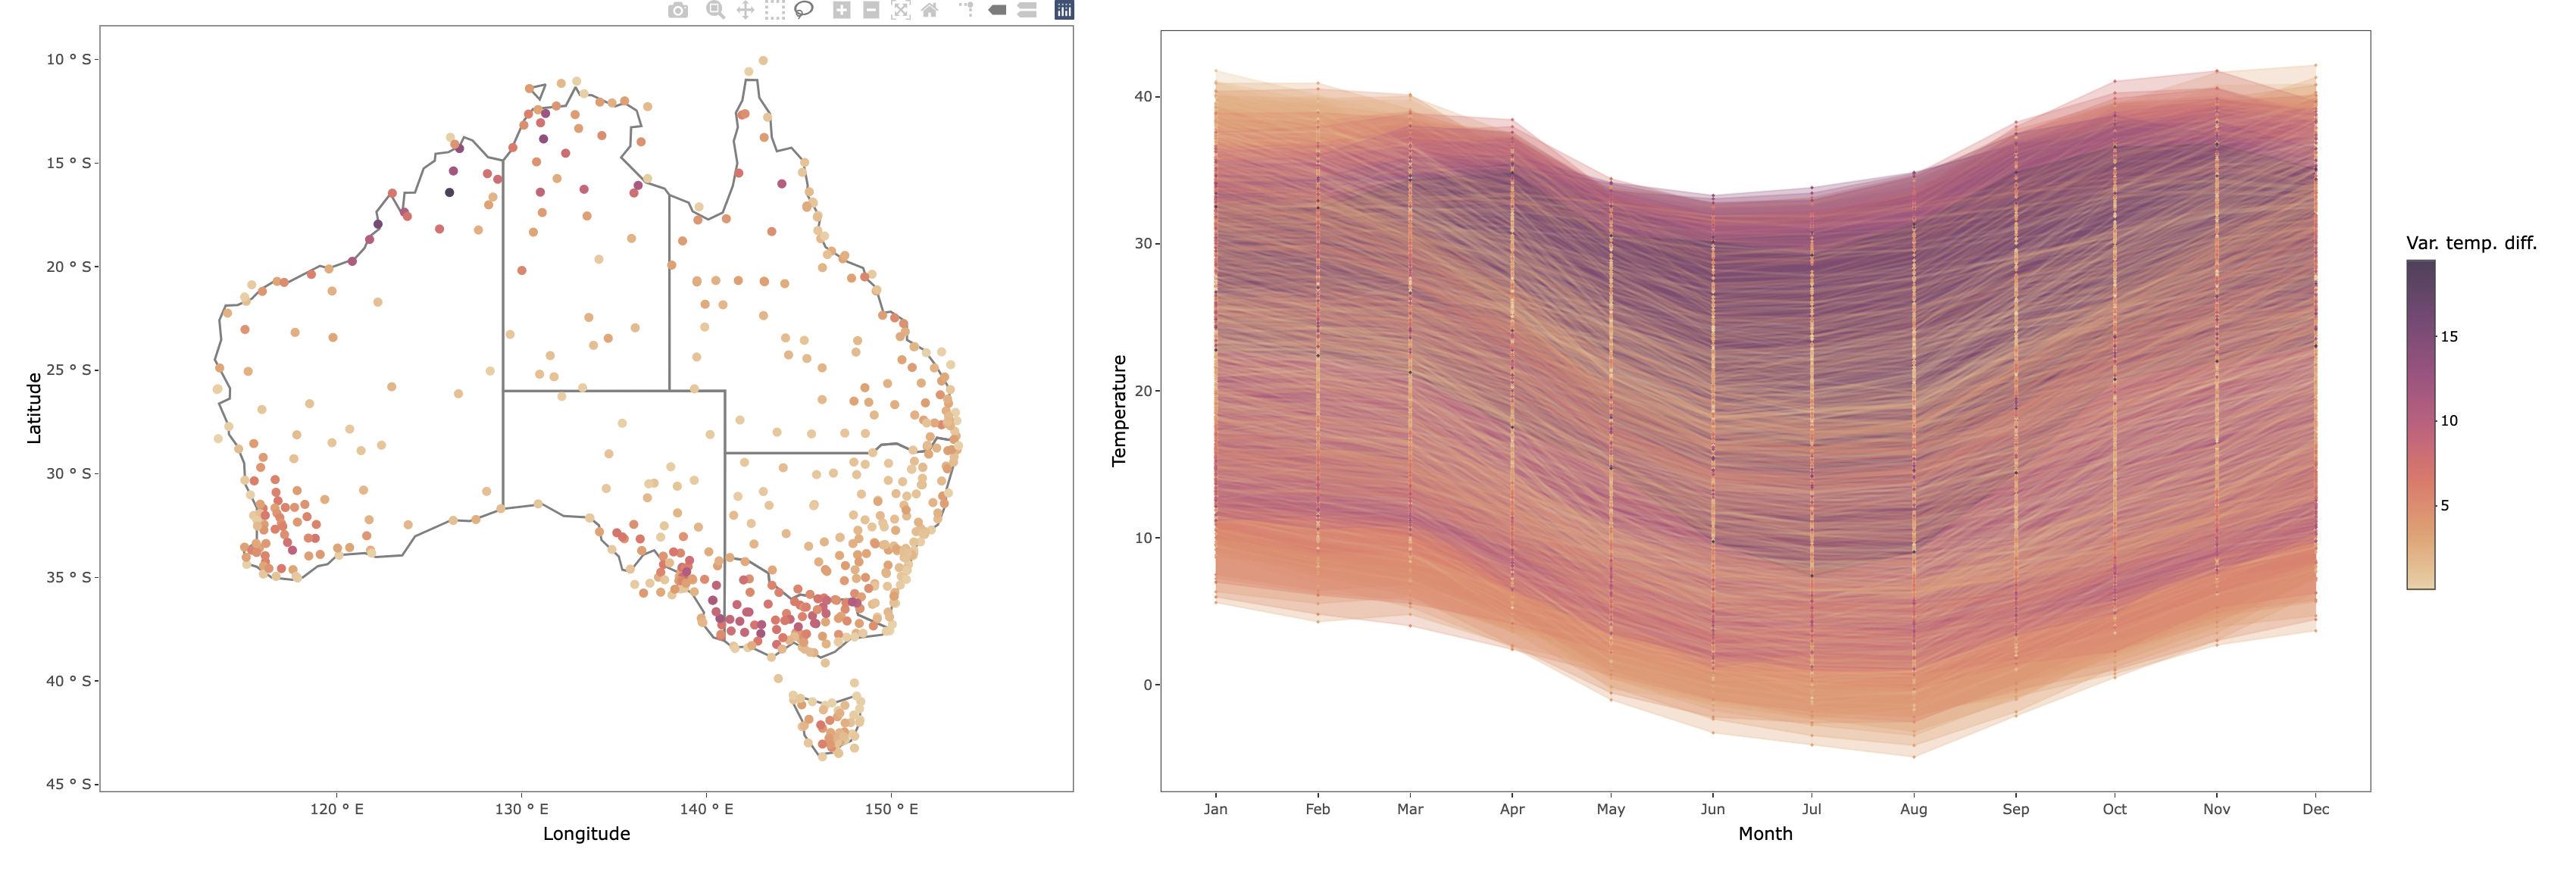
\includegraphics[width=1\linewidth,height=0.23\textheight]{figures/linking} 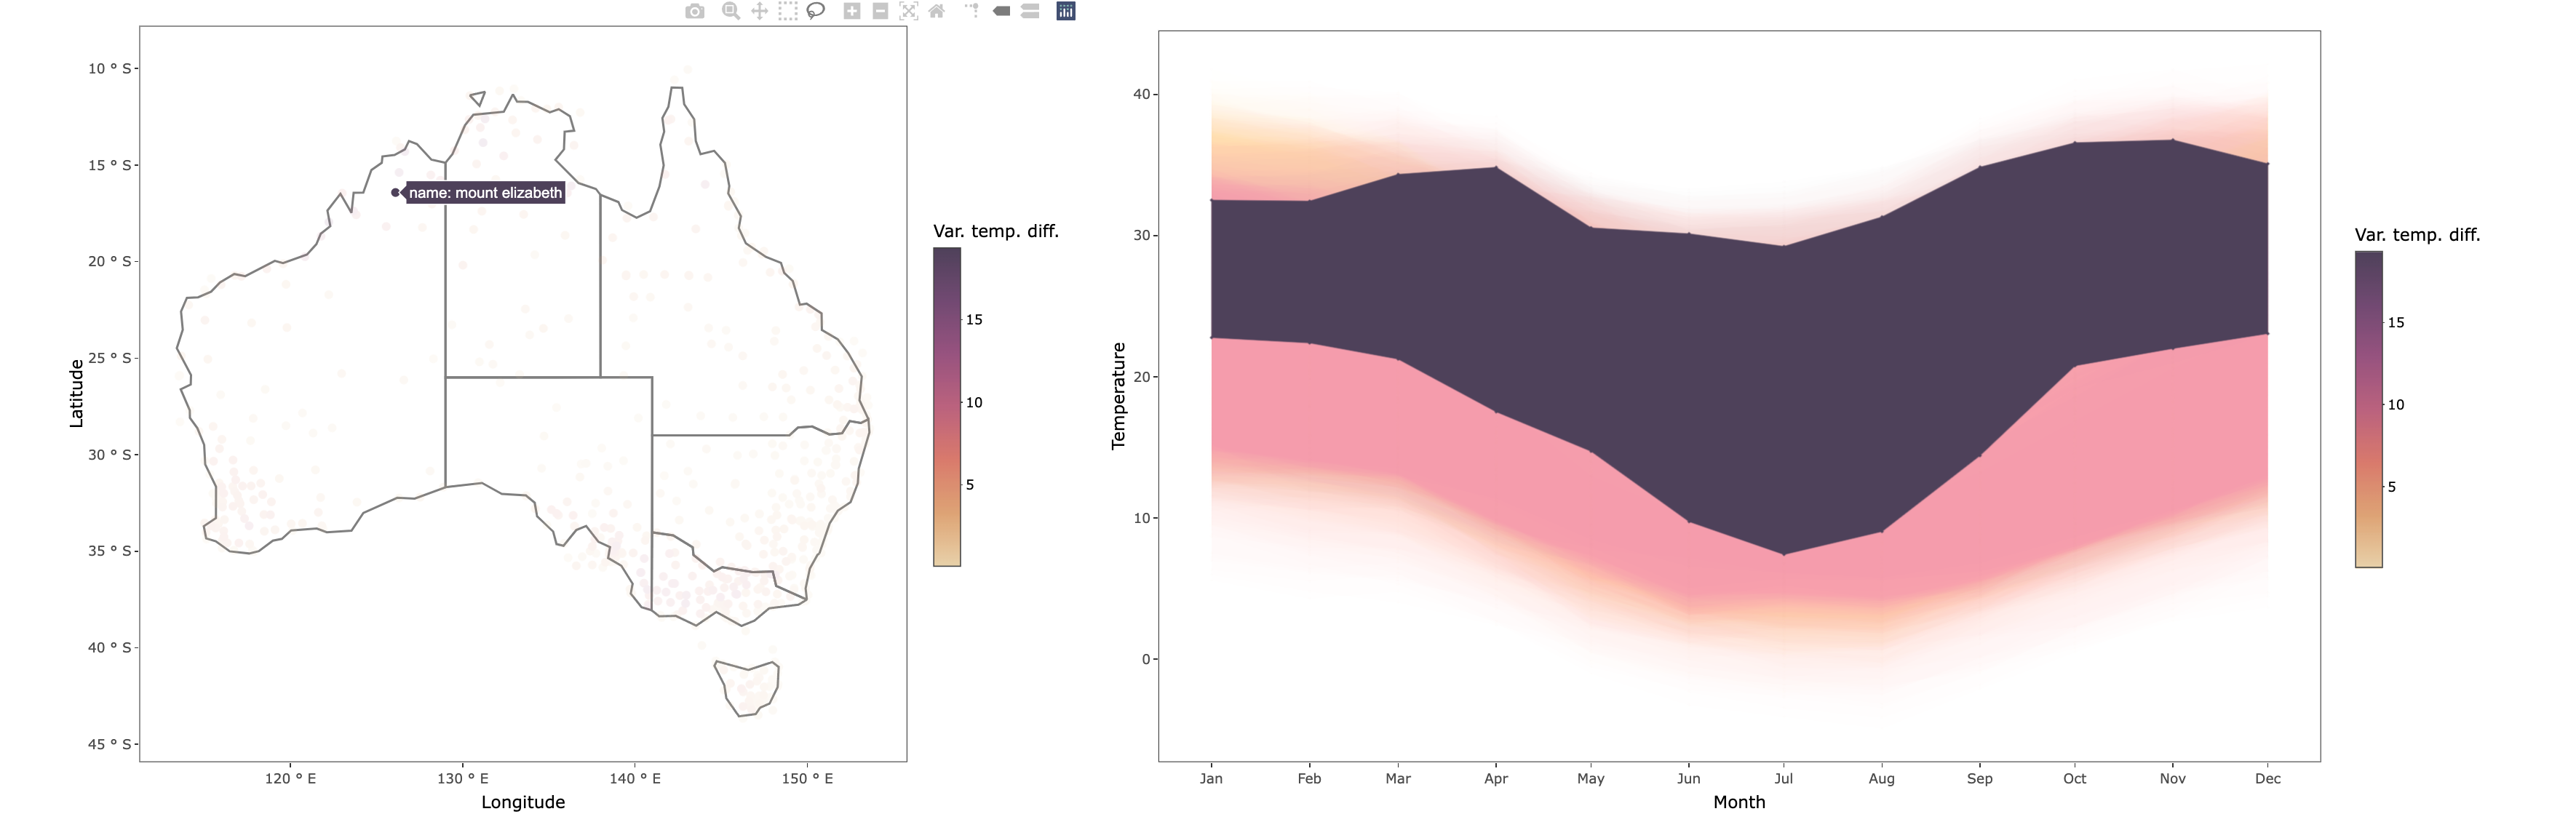
\includegraphics[width=1\linewidth,height=0.23\textheight]{figures/linking-north} 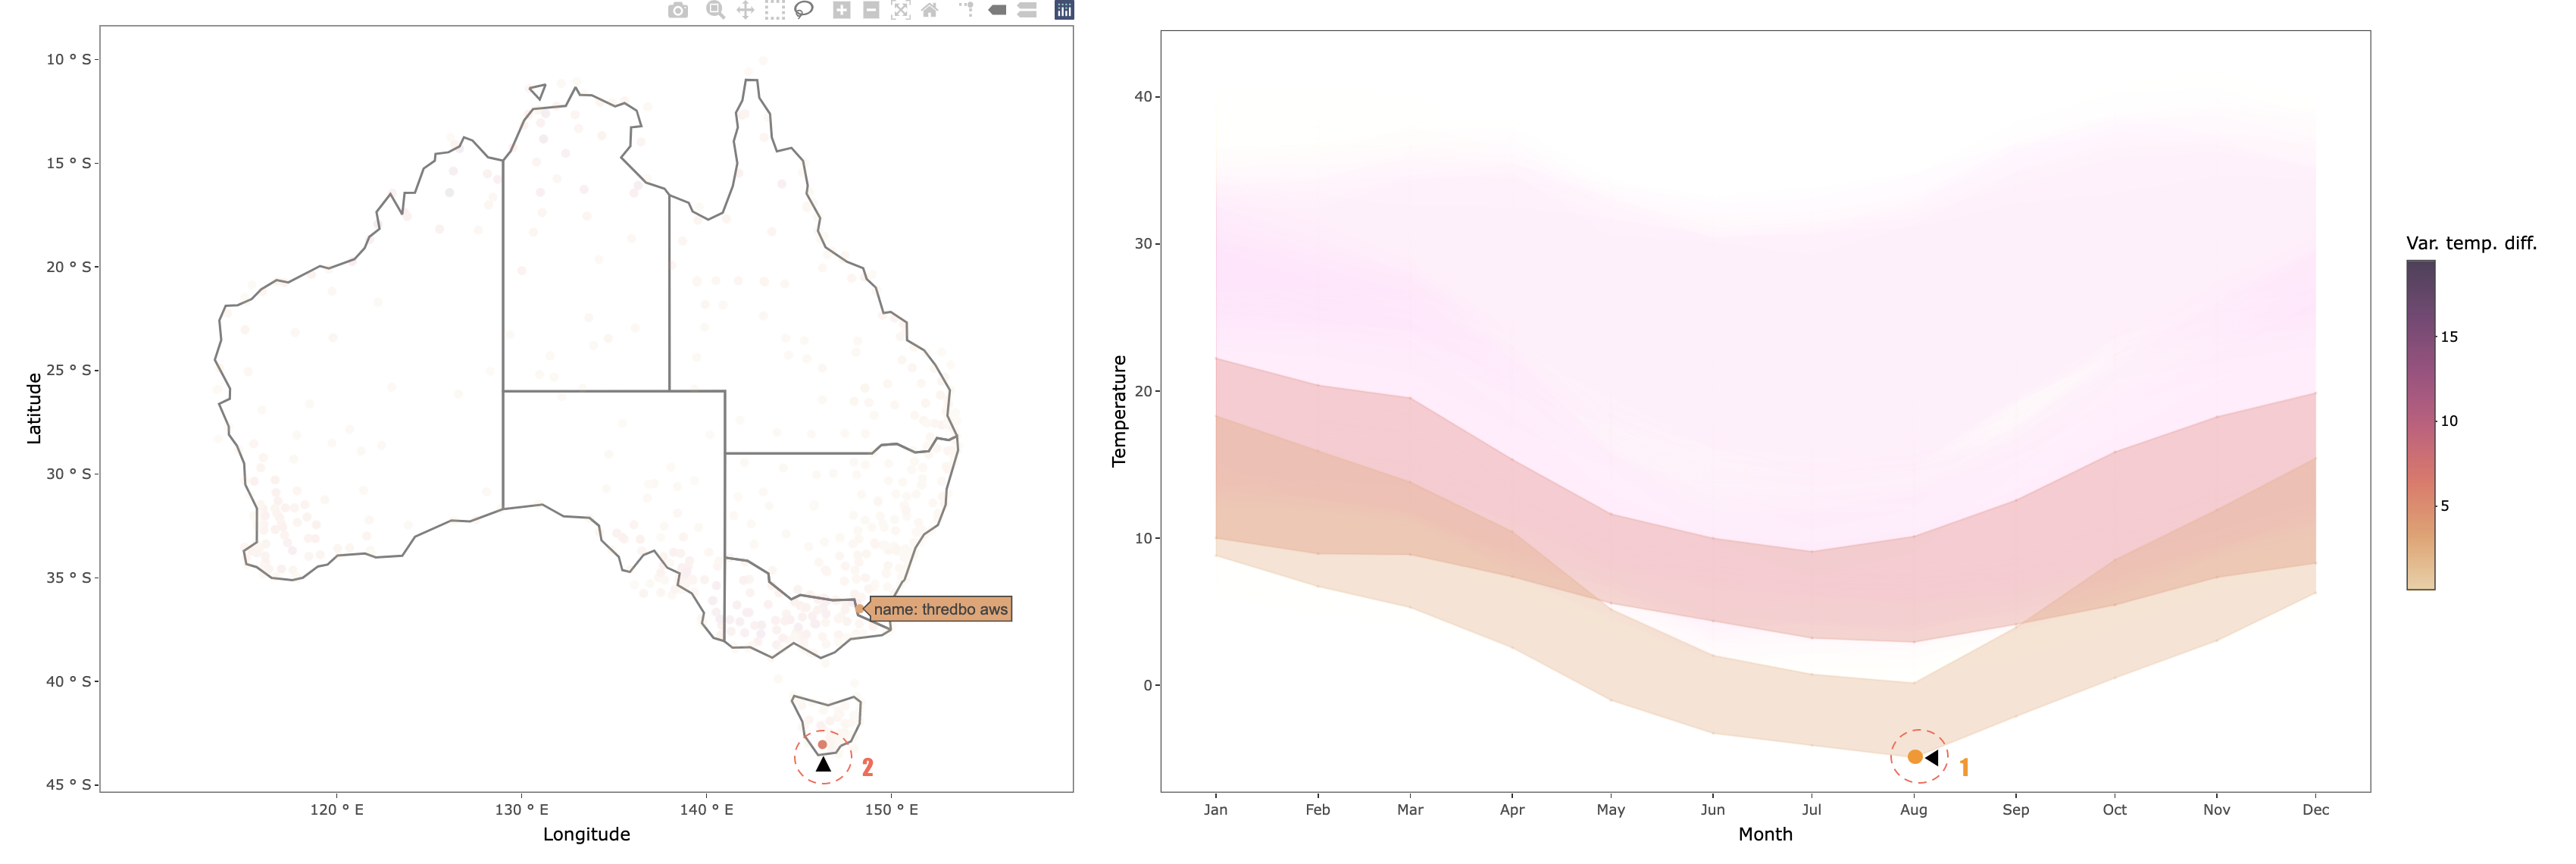
\includegraphics[width=1\linewidth,height=0.23\textheight]{figures/linking-lower} 

}

\caption[Exploring temperature variation using linking of a map and seasonal display]{Exploring temperature variation using linking of a map and seasonal display. Each row is a screen dump of the process. The top row shows all locations and all temperature profiles. Selecting a particular location on the map (here Mount Elizabeth) produces the plot in the second row. The maximum and minimum temperatures are shown using a ribbon. The bottom row first selects the lowest temperature in August in the seasonal display, which highlights the corresponding station on the map (Thredbo). Another  station, located in the Tasmania Island, is then selected to compare its temperature variation with the Thredbo station.}\label{fig:interactive-linking}
\end{figure}
\end{CodeChunk}

\hypertarget{conclude}{%
\section{Conclusion}\label{conclude}}

This paper presents the \proglang{R} package \pkg{cubble} for organizing, wrangling and visualizing spatio-temporal data. The package introduces a new data class, \code{cubble}, consisting of two subclass, spatial cubble and a temporal cubble, to organise spatio-temporal data in two different formats within the tidy data framework. The data structure and functions introduced in this package can be used and combined with existing spatial and temporal data analysis packages such as \pkg{sf} and \pkg{tsibble}, data wrangling packages such as \pkg{dplyr}, and visualization packages such as \pkg{ggplot2}, \pkg{plotly}, and \pkg{leaflet}.

The paper includes numerous examples to illustrate the utility of \pkg{cubble} as a data structure for spatio-temporal analysis. These examples cover different tasks of a typical analysis workflow: handling data with spatial and temporal misalignment, matching data from multiple sources, and creating both static and interactive spatio-temporal visualisation. For future directions, other commonly-used spatial or temporal data structures can be integrated into \pkg{cubble} to extend analysts' familiar spatial and temporal toolkit to spatio-temporal.

\hypertarget{acknowledgement}{%
\section{Acknowledgement}\label{acknowledgement}}

This work is funded by a Commonwealth Scientific and Industrial Research Organisation (CSIRO) Data61 Scholarship and started while Nicolas Langrené was affiliated with CSIRO's Data61. The article is created using the package \pkg{knitr} \citep{knitr} and \pkg{rmarkdown} \citep{rmarkdown} in \proglang{R} with the \code{rticles::jss_article} template. The source code for reproducing this paper can be found at: \url{https://github.com/huizezhang-sherry/paper-cubble}.

\bibliography{references.bib}



\end{document}
